\documentclass[12pt]{article}
\usepackage{graphicx} % Required for inserting images
\usepackage{mathptmx}
\usepackage{amsmath}
\usepackage{fontspec}
\usepackage{setspace}
\usepackage[a4paper, total={6in, 9in}]{geometry}
\usepackage{caption}
\usepackage{ragged2e}
\usepackage{tabularx}
\usepackage{subcaption}
\usepackage{float}
\usepackage{amssymb}
\usepackage[style=mla]{biblatex}
\usepackage{fancyhdr}
\usepackage[titletoc]{appendix}
\setmainfont{Arial}
\pagestyle{fancy}

% Customize footer
\fancyhf{} % Clear all headers and footers
\fancyfoot[C]{\small\thepage} % Small page number in center footer
\renewcommand{\headrulewidth}{0pt} % No header line
\renewcommand{\footrulewidth}{0pt} % No footer line

\doublespacing
\DeclareCaptionFormat{underlined}{\underline{\text{#1#2#3}}}
\captionsetup[figure]{format=underlined,labelformat=simple,labelsep=colon}
\captionsetup[table]{format=underlined,labelformat=simple,labelsep=colon}
\addbibresource{bibliography.bib}

\begin{document}

\setlength\parindent{0pt}
\setlength{\footskip}{1in} % dist between page no. and text
\addtolength{\jot}{1em}% spacing between equations

In primary school, I was taught that Singapore was a "little red dot". This memory has stuck with me throughout the years, which has inspired me to investigate how big Singapore truly is. Accurate estimations of the area of Singapore (AOS) can provide useful information about the country's population density, building density and the country's progress on land reclamation among other useful statistics \parencite{land_auth}.\newline

In this investigation, a map of Singapore shown in figure \ref{fig:map} will be used. The AOS is defined as the area of the main island of Singapore, including the bodies of water that run through the island. Bodies of water are indicated by the blue areas on the map. In order to find the AOS, different methods of calculating areas on a graph will be used, such as the Shoelace Method and integration. Each method used will attempt to enhance the accuracy of the approximated AOS from the previous method by addressing considerable drawbacks, ensuring that the concluded AOS will be as close to the actual value of the AOS as possible.\newline

\begin{figure}[H]
    \centering
    \caption{Map of Singapore}
    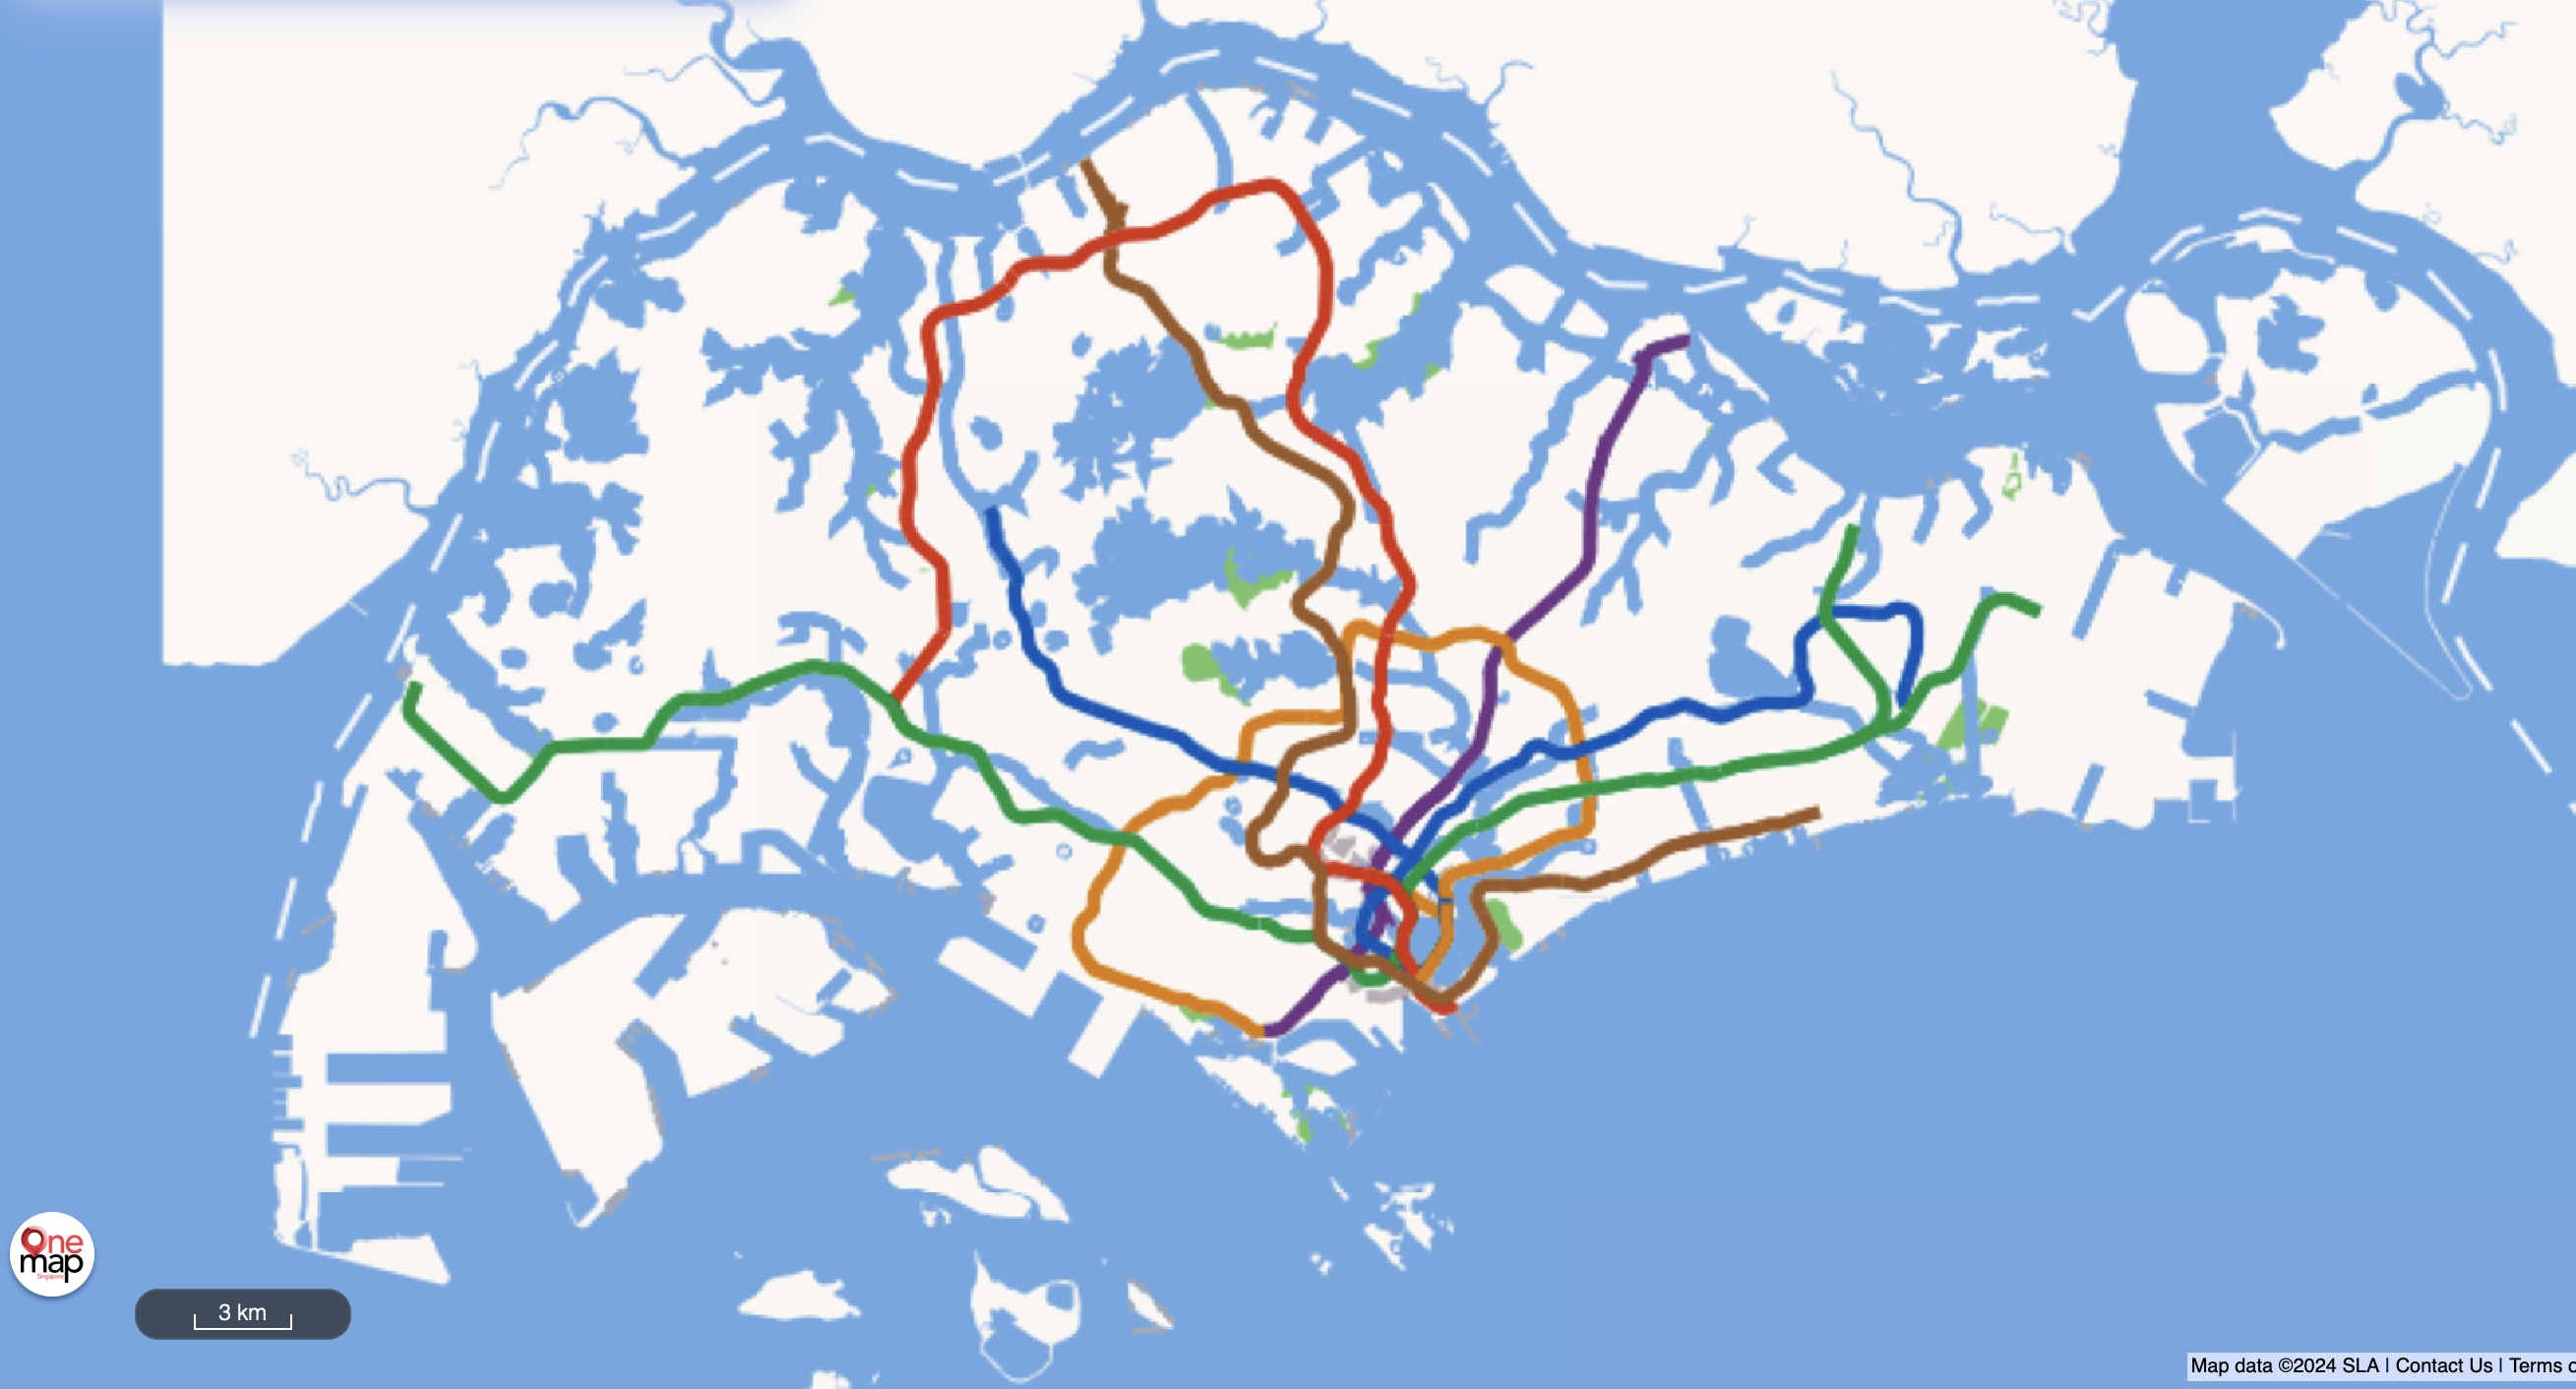
\includegraphics[width=0.9\linewidth]{media/map.jpeg}
    \textit{Source: https://www.onemap.gov.sg/}
    \label{fig:map}
\end{figure}

In order to estimate the AOS, I first utilised basic geometry to draw rectangles and triangles on the map of Singapore and finding their respective areas.\newline

\begin{figure}[H]
    \centering
    \caption{Using basic shapes to estimate AOS}
    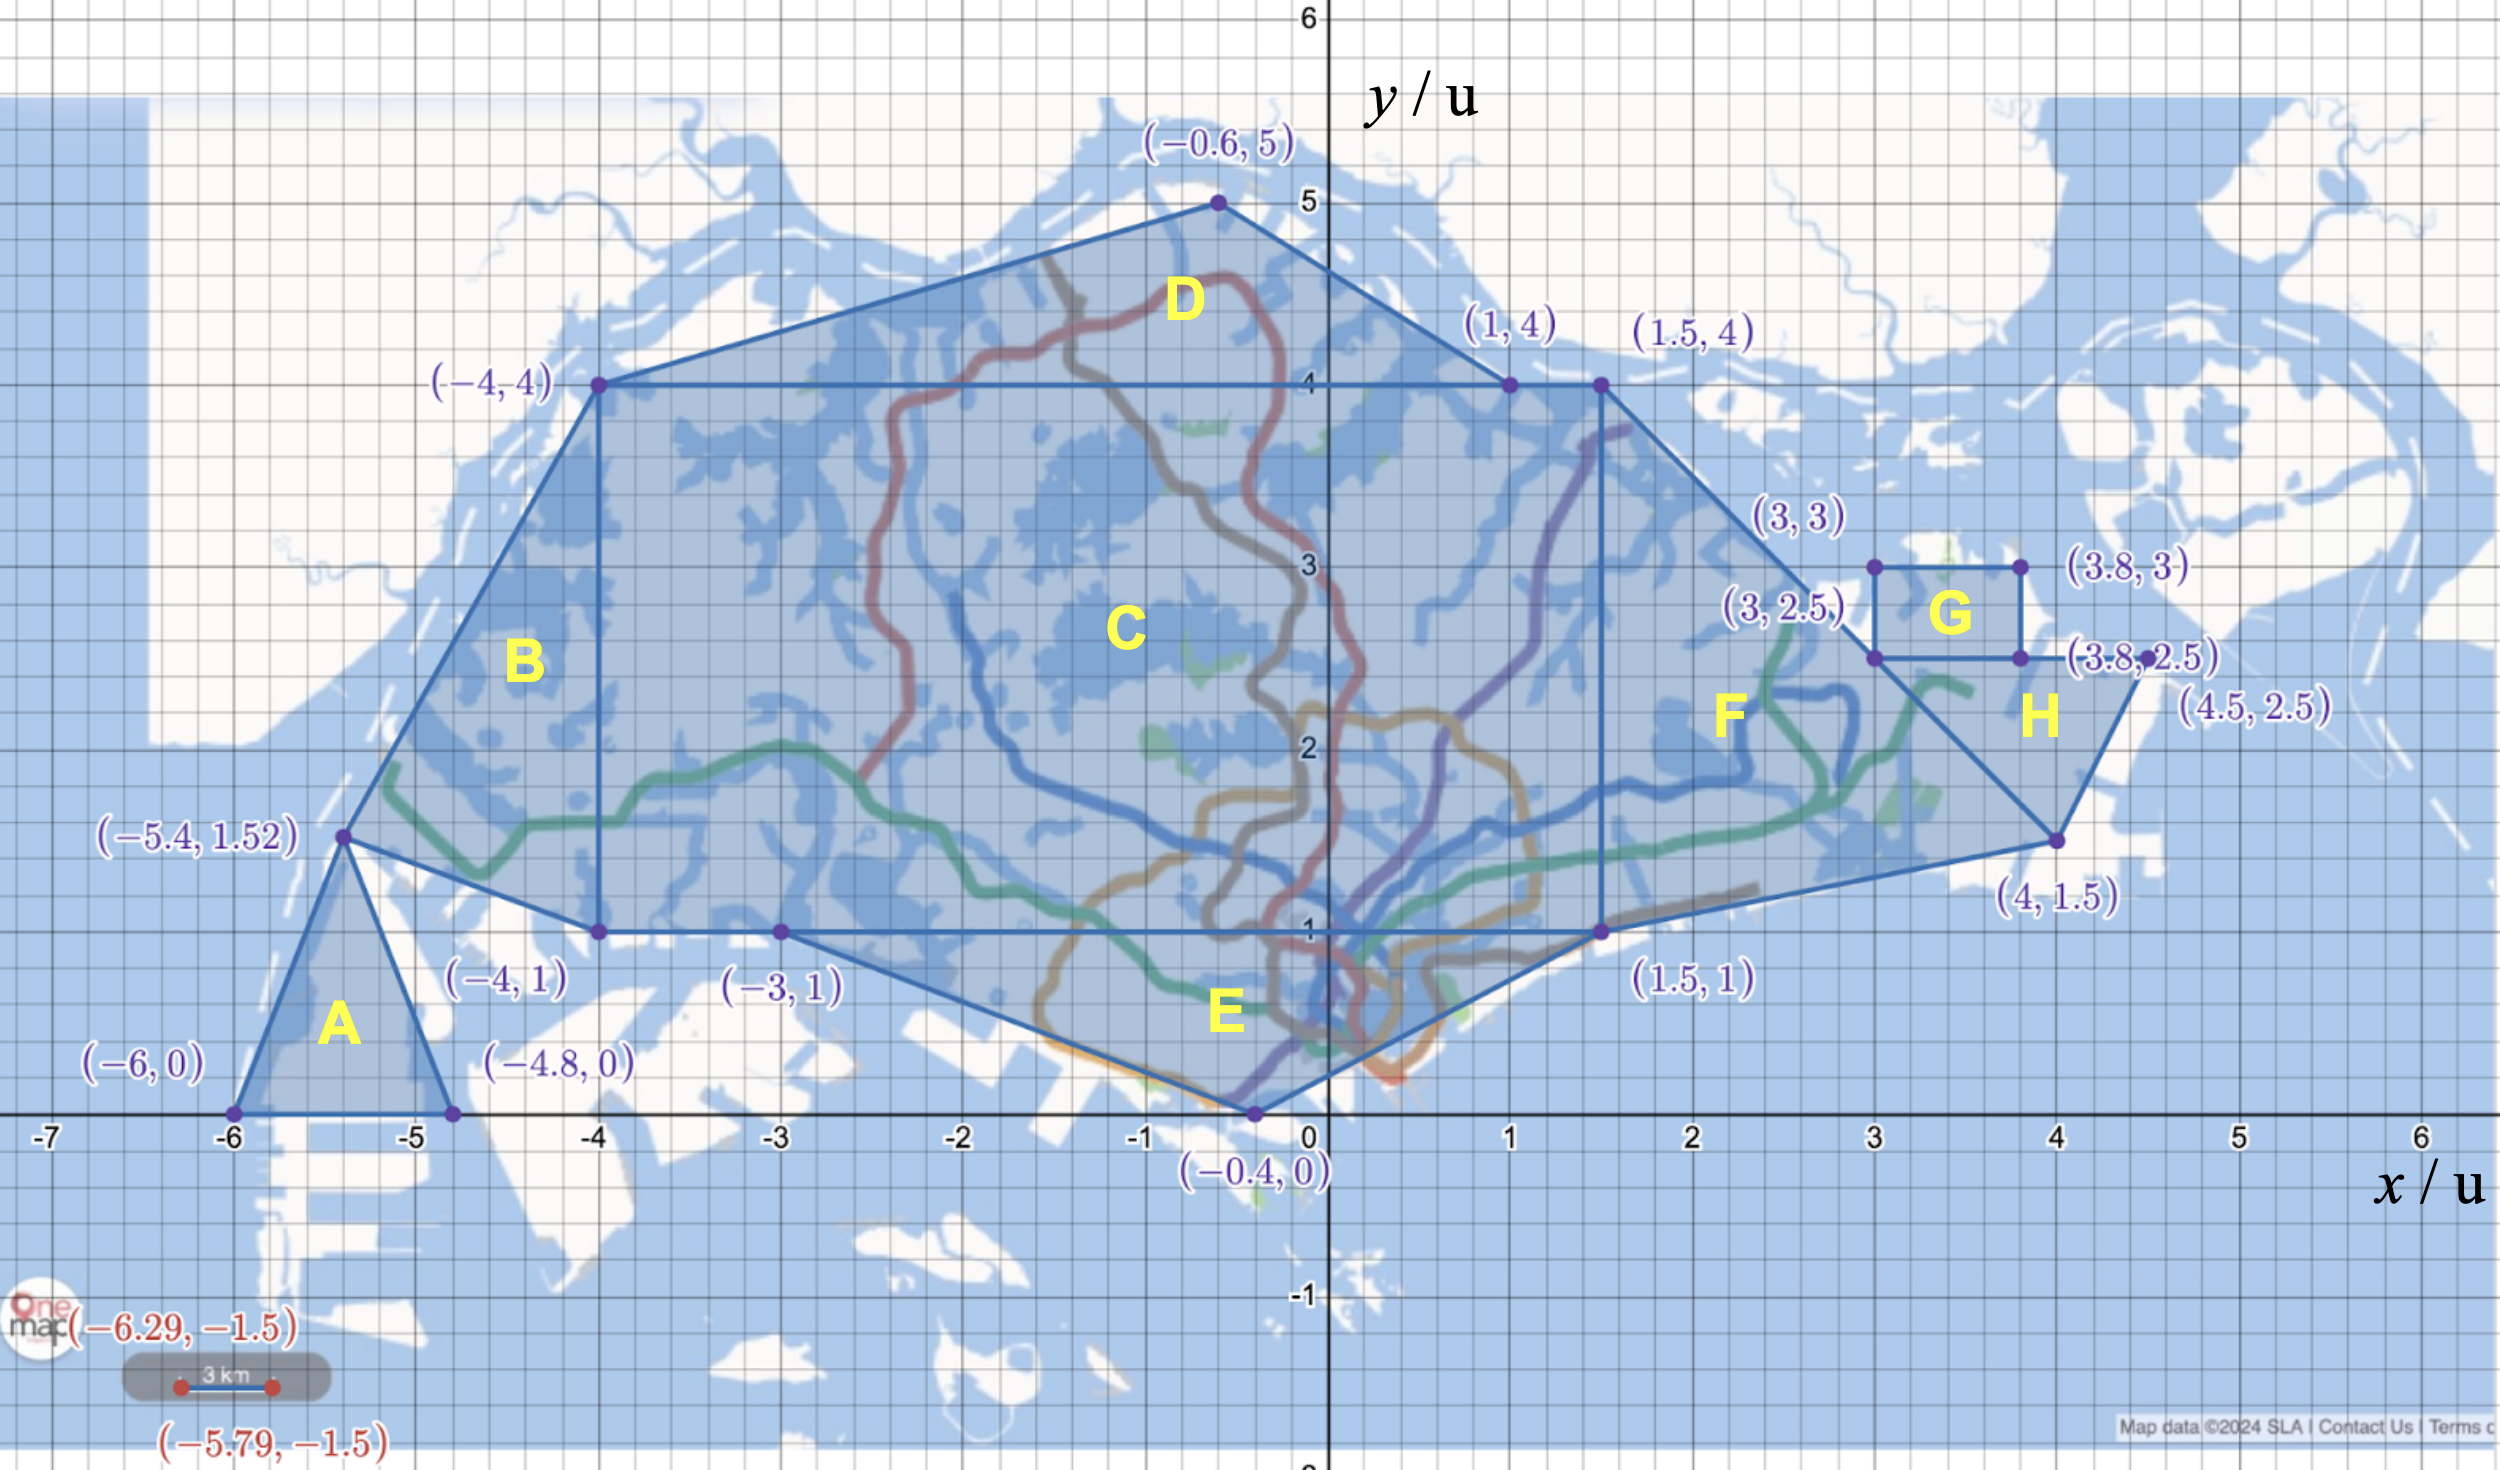
\includegraphics[width=0.9\linewidth]{media/simple-shapes-units.png}
    \label{fig:basic_shapes}
\end{figure}

In figure \ref{fig:basic_shapes}, a grid with an $x$ and $y$ axis is transposed onto the map of Singapore from figure \ref{fig:map}. The ratio between lengths on the grid in Desmos (u) and the actual distances in kilometres (km) is $0.5:3$. This ratio is calculated by placing the map's bar scale horizontally, in between the lines of $x=-6.29$ and $x=-5.79$, inclusive. As a result, the map's bar scale of $3$ km fits into a region that is $0.5$ u wide.\newline

There are a total of eight polygons drawn, consisting of rectangles and triangles. To estimate the AOS, I will utilise the formulas for the area of a triangle and an area of a rectangle with the coordinates of each polygon. The sum of all areas will then be converted from u to km.
\newpage

According to the \cite{ib},
\bgroup
\singlespacing
\begin{align*}
    \text{Area of a rectangle}&= \text{base} \times \text{height}\\
    \text{Area of a triangle} &= \frac{1}{2}\times\text{base}\times\text{height}
\end{align*}
\egroup

In order to calculate the base of a rectangle or triangle from figure \ref{fig:basic_shapes}, I would take two of its coordinates that have the same $y$-value and find the difference between their $x$-values. To find the height, the difference in the maximum and minimum $y$-value of any two coordinates that form the shape will be calculated.

\bgroup
\singlespacing
\allowdisplaybreaks
\begin{align*}
    \text{Area of A} &= \frac{1}{2}\times(-4.8-(-6))\times1.52\\
    &=0.912 \text{ u}^2\\
    \text{Area of B} &= \frac{1}{2}\times(4-1)\times(-4-(-5.4))\\
    &=2.1 \text{ u}^2\\
    \text{Area of C} &= (1.5-(-4))\times(4-1)\\
    &=16.5 \text{ u}^2\\
    \text{Area of D} &= \frac{1}{2}\times(1-(-4))\times(5-4)\\
    &=2.5 \text{ u}^2\\
    \text{Area of E} &= \frac{1}{2}\times(1.5-(-3))\times1\\
    &=2.25 \text{ u}^2\\
    \text{Area of F} &= \frac{1}{2}\times(4-1)\times(4-1.5)\\
    &=3.75 \text{ u}^2\\
    \text{Area of G} &= (3.8-3)\times(3-2.5)\\
    &=0.4 \text{ u}^2\\
    \text{Area of H} &= \frac{1}{2}\times(4.5-3)\times(2.5-1.5)\\
    &=0.75 \text{ u}^2
\end{align*}
\egroup

Therefore, the AOS in $\text{u}^2$ would be $0.912+2.1+16.5+2.5+2.25+3.75+0.4+0.75=29.162$.\newline

Since the ratio between a value in km and a value in u is $3:0.5$,

\bgroup
\singlespacing
\begin{align*}
    0.5\times\text{value in km}&=3\times \text{value in u}\\
    \text{value in km}&=6\times \text{value in u}\\
    \text{value in km}^2&=6^2\times \text{value in u}^2\\
    \therefore \text{AOS in km}^2&=36\times 29.162\\
    &=1049.832\\
    &\approx1050
\end{align*}
\egroup

Unfortunately, I realised that this method of calculating the AOS was impractical due to the fact that triangles and rectangles are made up of a relatively small set of lines. This prevents fine adjustments around uneven coastlines, resulting in some land being unaccounted for. This is shown in figure \ref{fig:map-problems}, where the most significant unaccounted land regions are indicated by red rectangles. As a result, the approximation of the AOS being $1050$ km$^2$ is inaccurate and is most likely underestimating the actual value of the AOS.
\begin{figure}[H]
    \centering
    \caption{Unaccounted Land Areas}
    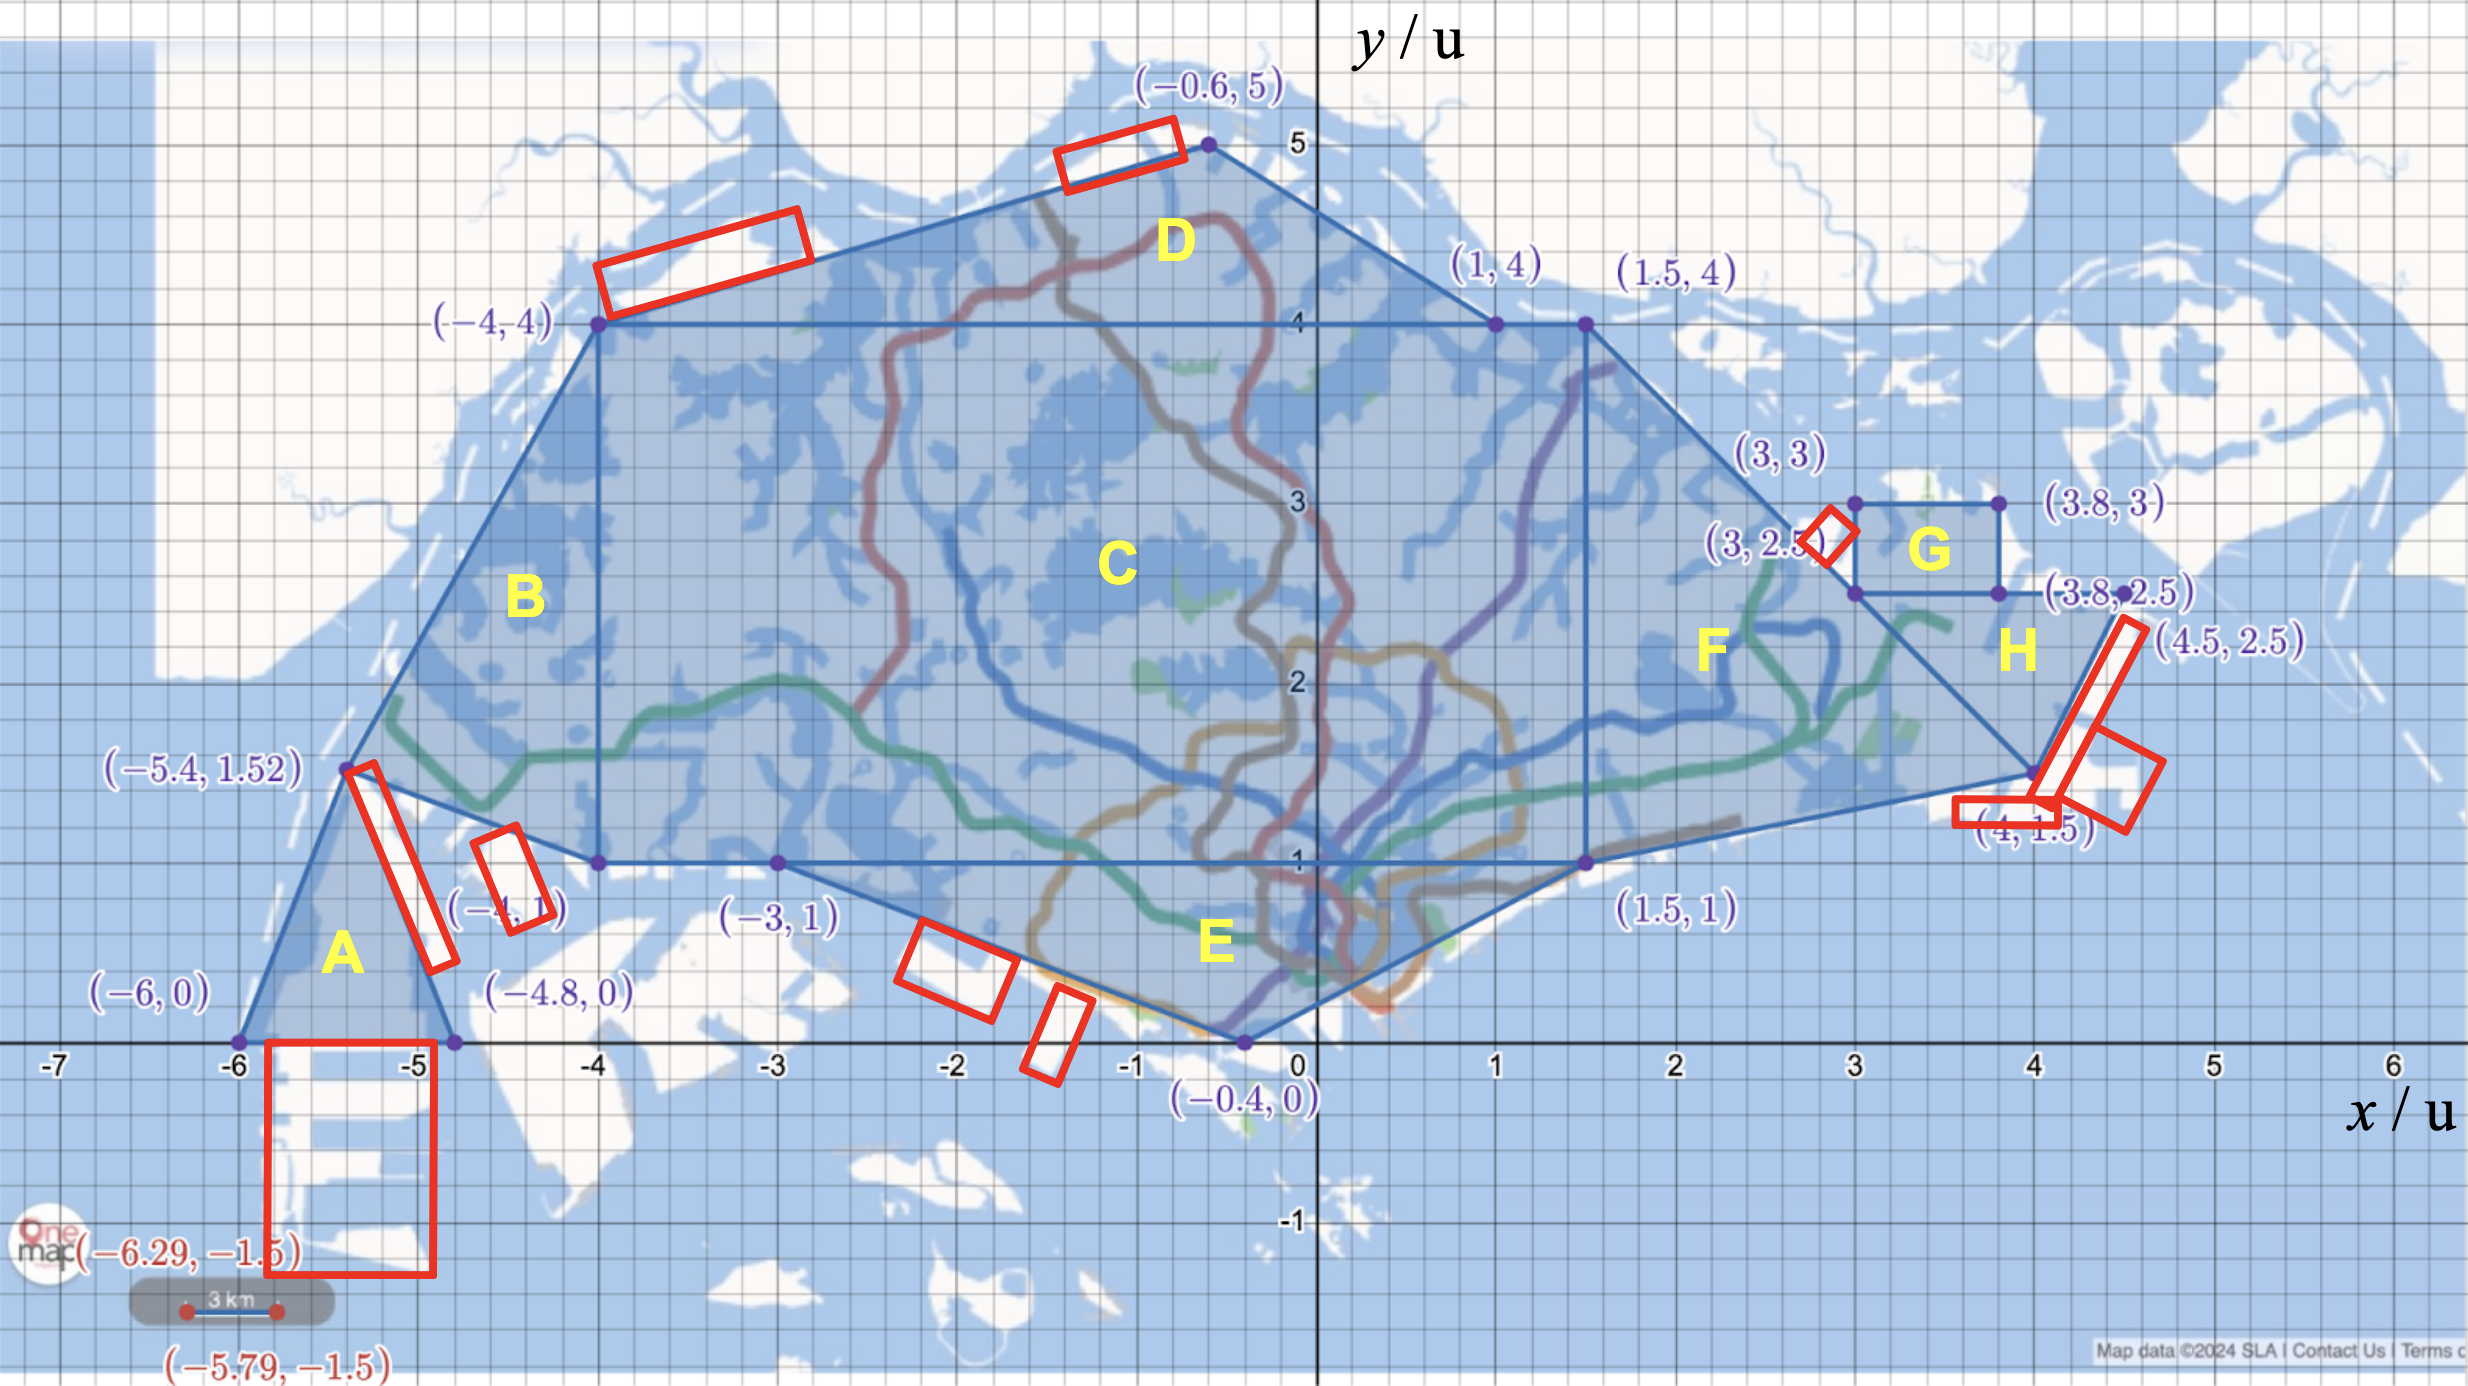
\includegraphics[width=0.8\linewidth]{media/shapes-problems-units.png}
    \label{fig:map-problems}
\end{figure}
In order to improve the approximated AOS, I decided to utilise the Shoelace method which would enable me to make finer adjustments to uneven coastlines and reduce the occurrences of miscounted bodies of water. In this investigation, bodies of water indicated by the blue areas in figure \ref{fig:map} that are within the coastline of Singapore will still be counted as part of the AOS due to the multiple rivers and reservoirs that make up Singapore.\newline

Finding the area of a $n$-sided polygon using the Shoelace method involves the use of a set of coordinates that make up said $n$-sided polygon, where coordinates are oriented clockwise or anticlockwise, where $n\in\mathbb{Z}^+$ \parencite{lee_shoelace}.\newline

According to \cite{lee_shoelace}, the formula for the shoelace theorem is given as:
\begin{equation} \label{eqn:shoelace-og}
    \text{A} = \frac{1}{2}|(x_1y_2+x_2y_3+\dots+x_ny_1)-(x_2y_1+x_3y_2+\dots+x_1y_n)|,\\
\end{equation}
where A is the area of an $n$-sided polygon, with $x_n$ and $y_n$ being the $x$ and $y$ values of the $n$th coordinate.

Equation \ref{eqn:shoelace-og} is derived from the summation of trapezoids. For explanation purposes, consider figure \ref{fig:shoe-0} below.

\begin{figure}[H]
    \centering
    \caption{Example scenario for the shoelace theorem}
    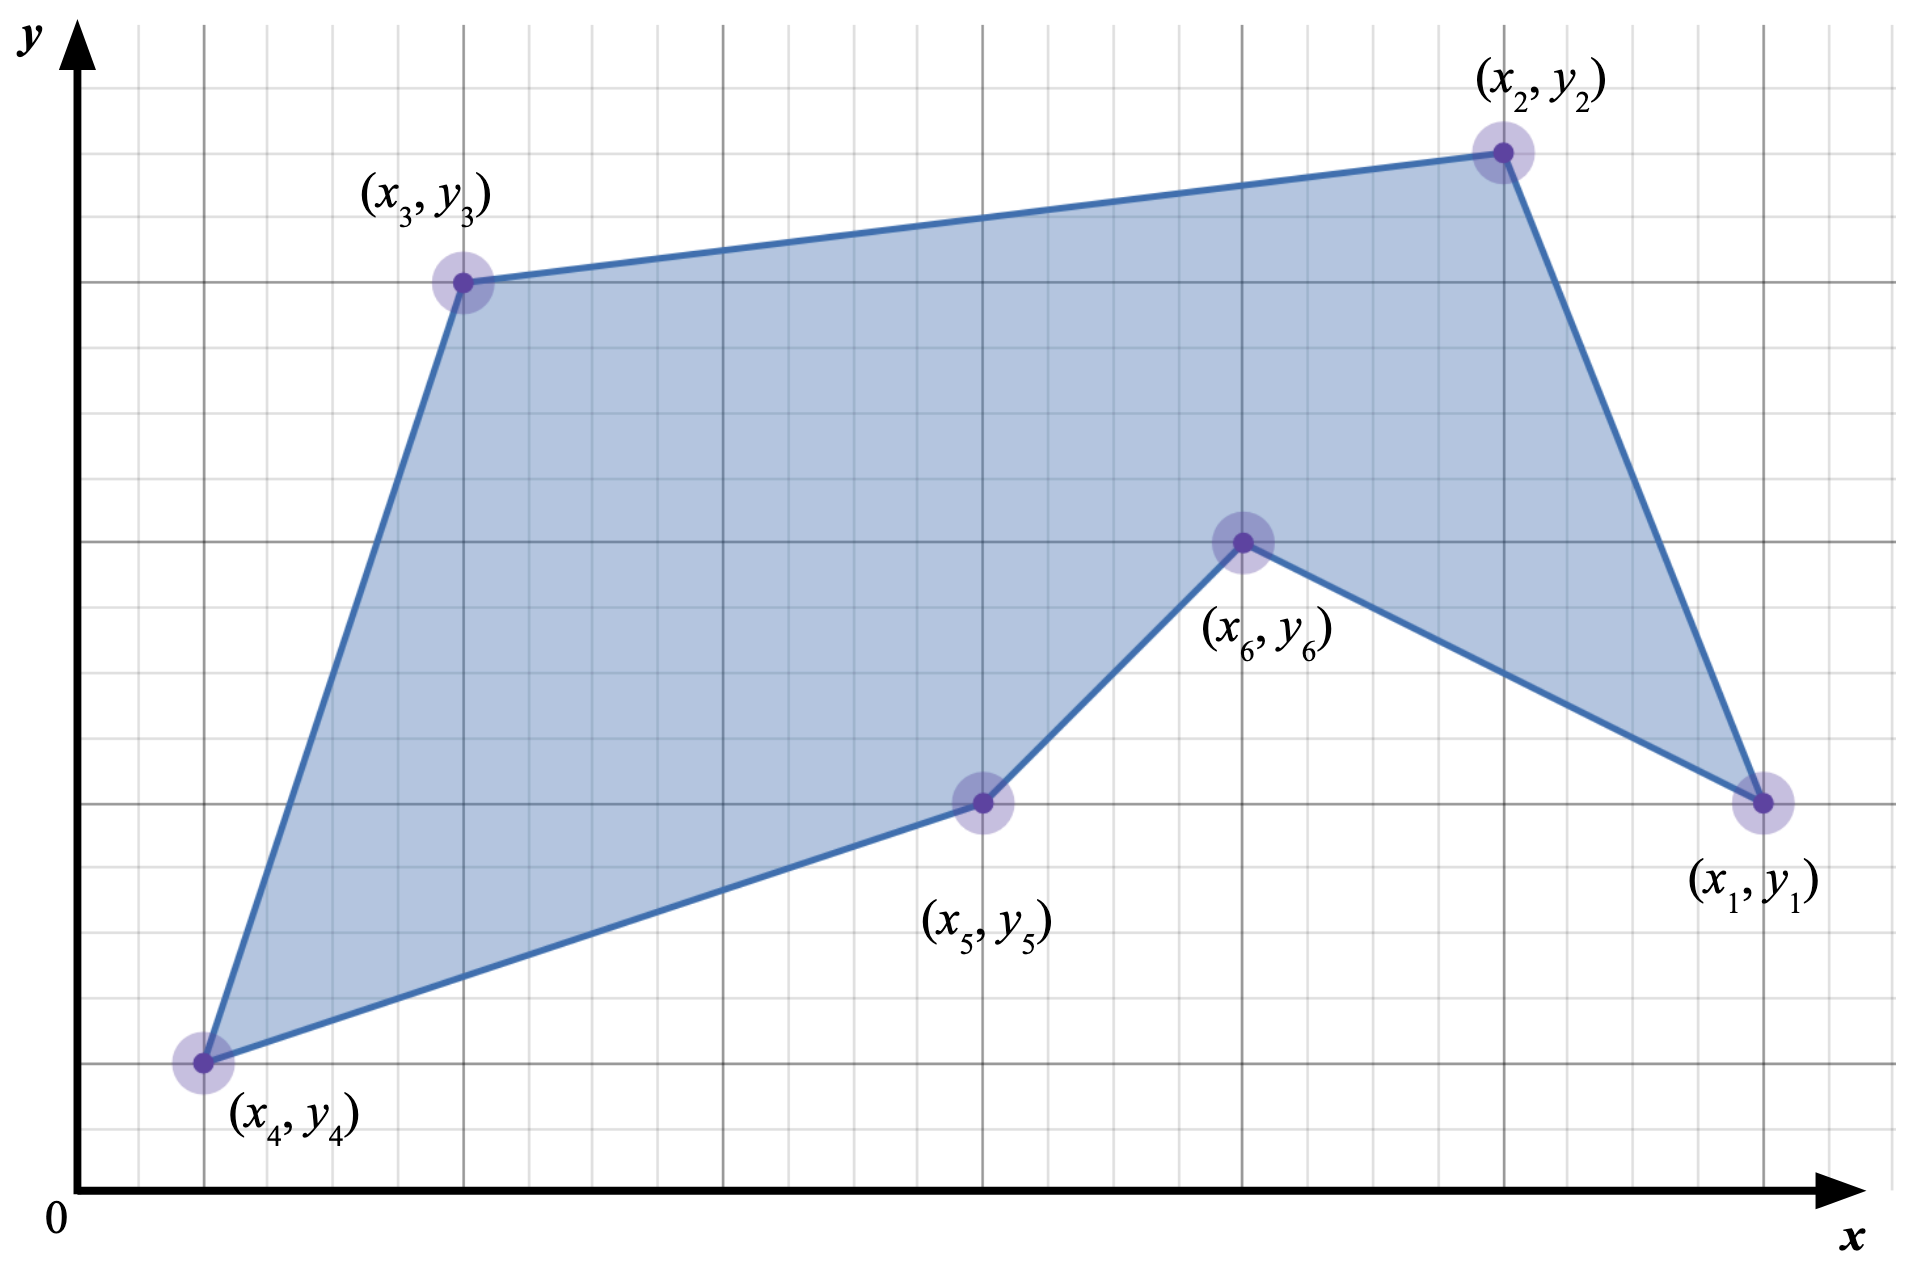
\includegraphics[width=0.8\linewidth]{media/shoelace/0-shoelace.png}
    \label{fig:shoe-0}
\end{figure}

In order to find the area of the shape in figure \ref{fig:shoe-0}, the area can first be intentionally over-calculate by including the area between the shape and the $x$-axis. This allows me to use the formula for the area of a trapezoid,
\begin{equation}\label{eqn:trapezoid}
    A=\frac{1}{2}(a+b)h,\quad a,b,h\in \mathbb{R}^+
\end{equation}
where $a$ and $b$ represent the lengths of the respective parallel sides of the trapezoid and where $h$ is the height of the trapezoid \parencite{ib}. Below, equation \ref{eqn:trapezoid} is applied to the example scenario from figure \ref{fig:shoe-0}.

\begin{figure}[H]
    \centering
    \caption{Area of the first trapezoid of the over-calculated area}
    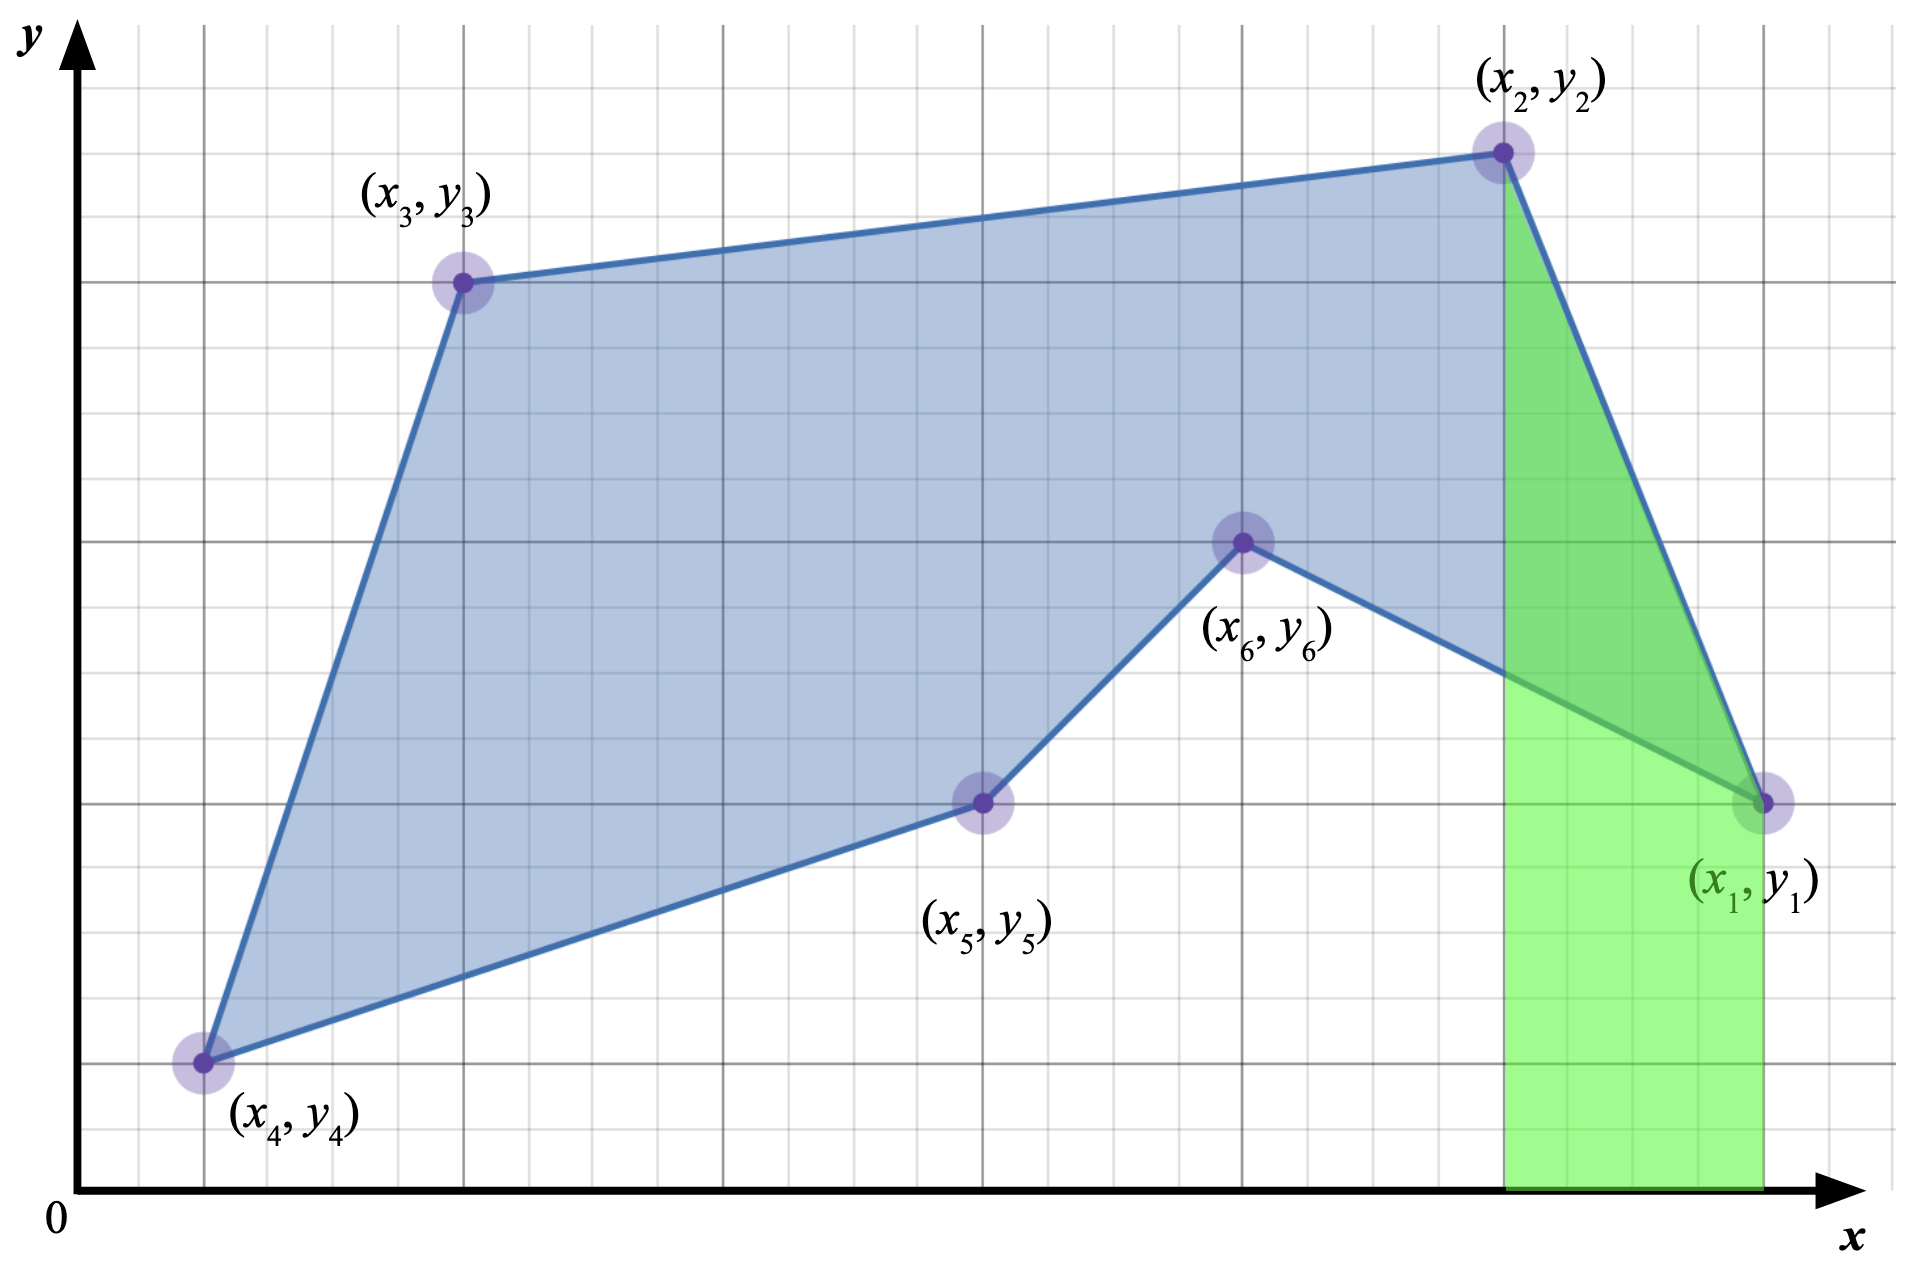
\includegraphics[width=0.8\linewidth]{media/shoelace/1-shoelace.png}
    \label{fig:shoe-1}
\end{figure}

With reference to figure \ref{fig:shoe-1}, I begin by calculating the area of the green region. Since it is a trapezoid with two parallel sides along the $y$-axis, I can apply equation \ref{eqn:trapezoid} to find its area:

\bgroup
\allowdisplaybreaks
\singlespacing
\begin{align*}
    \text{Recall from equation \ref{eqn:trapezoid}, }A&=\frac{1}{2}(a+b)h,\quad a,b,h\in \mathbb{R}^+\\
    a&=y_1\\
    b&=y_2\\
    h&=x_1-x_2\\
    \therefore \text{Area of green region in figure \ref{fig:shoe-1}}&=\frac{1}{2}(y_1+y_2)(x_1-x_2)
\end{align*}
\egroup

This process of over-calculating the area by including the region between the shape and the $x$-axis as well as the area of the shape itself in order to use the formula for the area of a trapezoid is repeated two more times so that the rest of the shape's area is accounted for, as shown in figures \ref{fig:shoe-2} and \ref{fig:shoe-3}.\newline

\begin{figure}[H]
    \centering
    \caption{Area of the second trapezoid of the over-calculated area}
    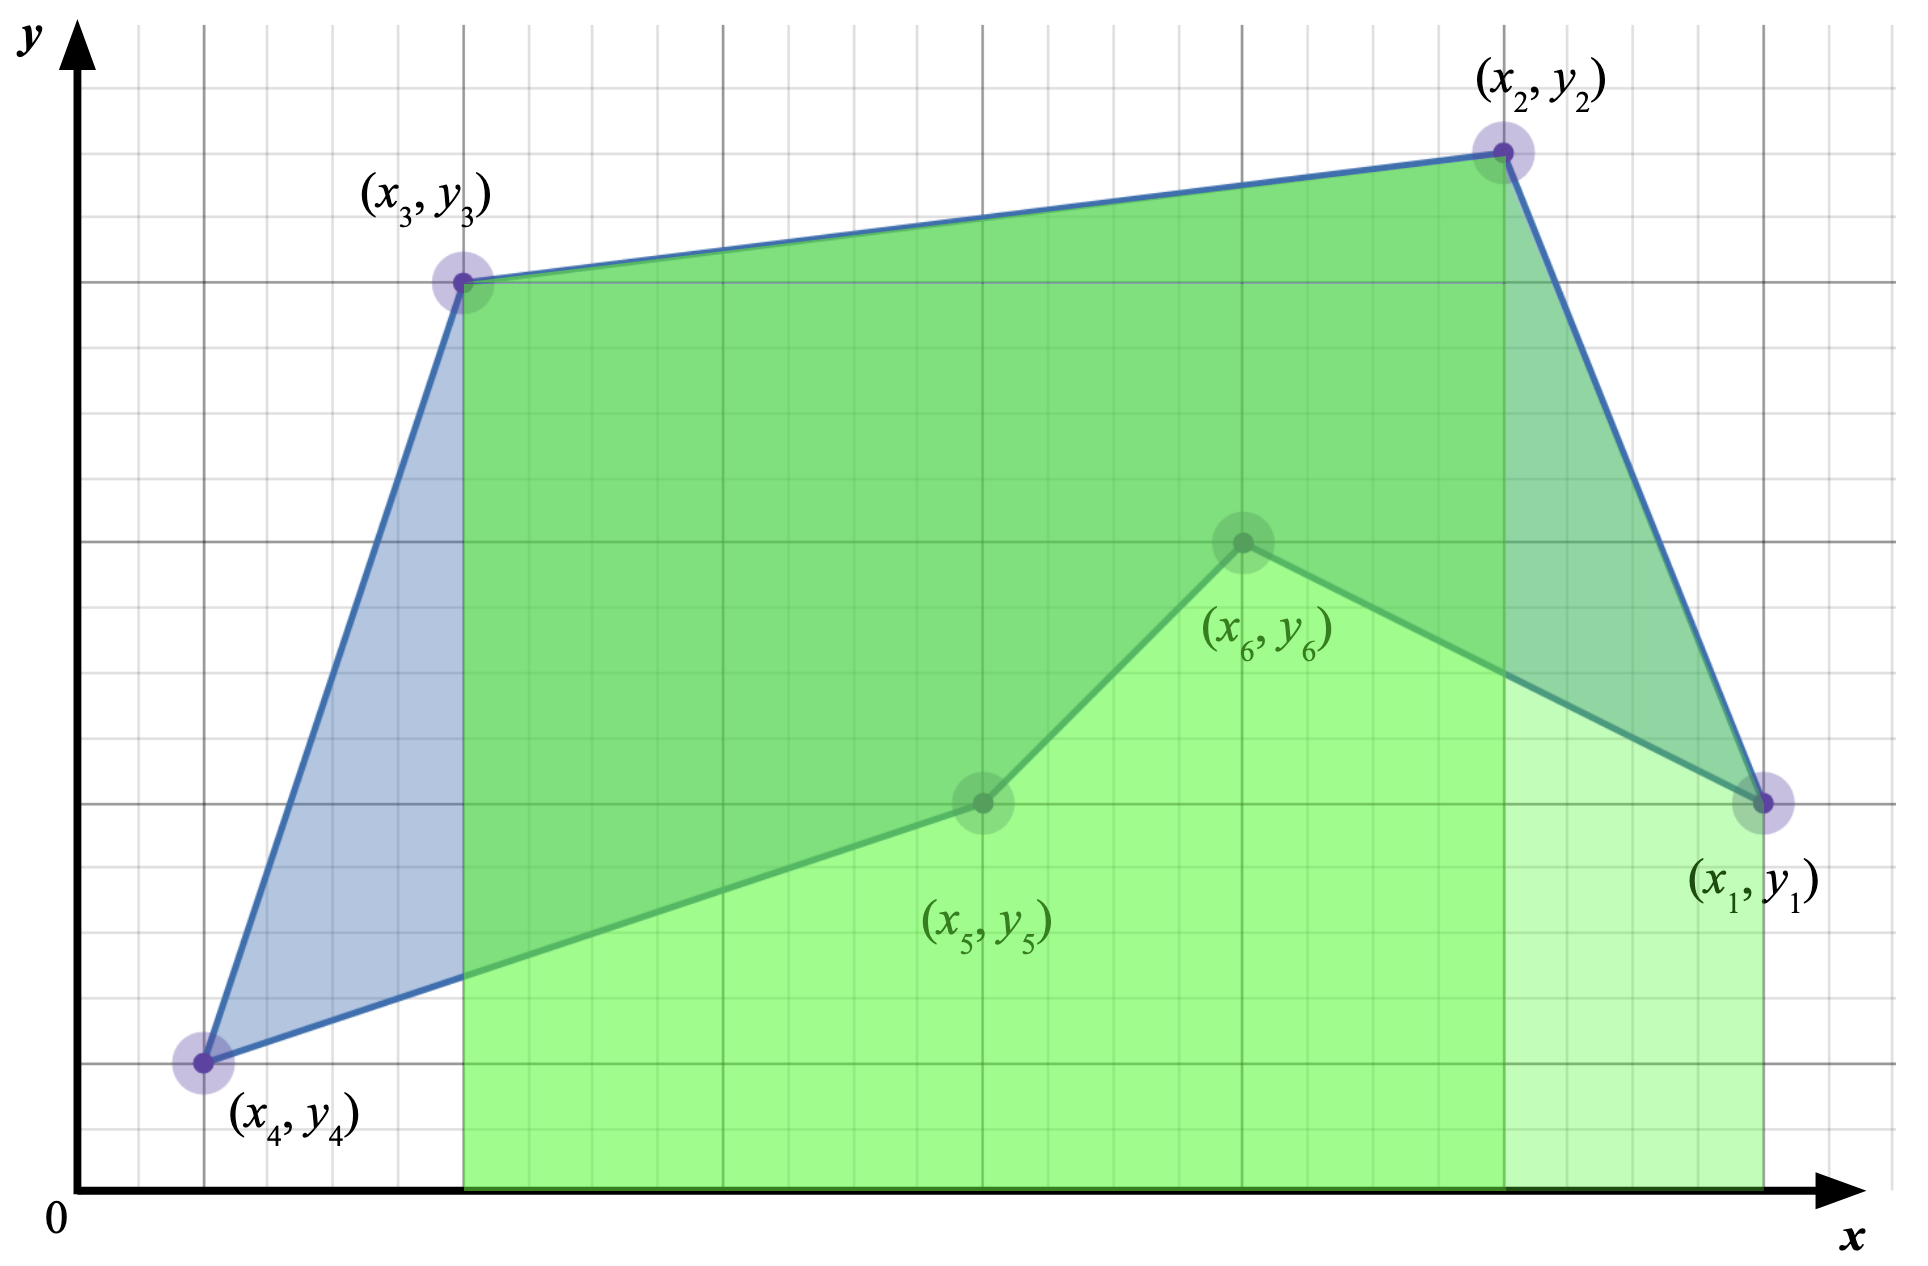
\includegraphics[width=0.8\linewidth]{media/shoelace/2-shoelace.png}
    \label{fig:shoe-2}
\end{figure}

\begin{figure}[H]
    \centering
    \caption{Area of the third trapezoid of the over-calculated area}
    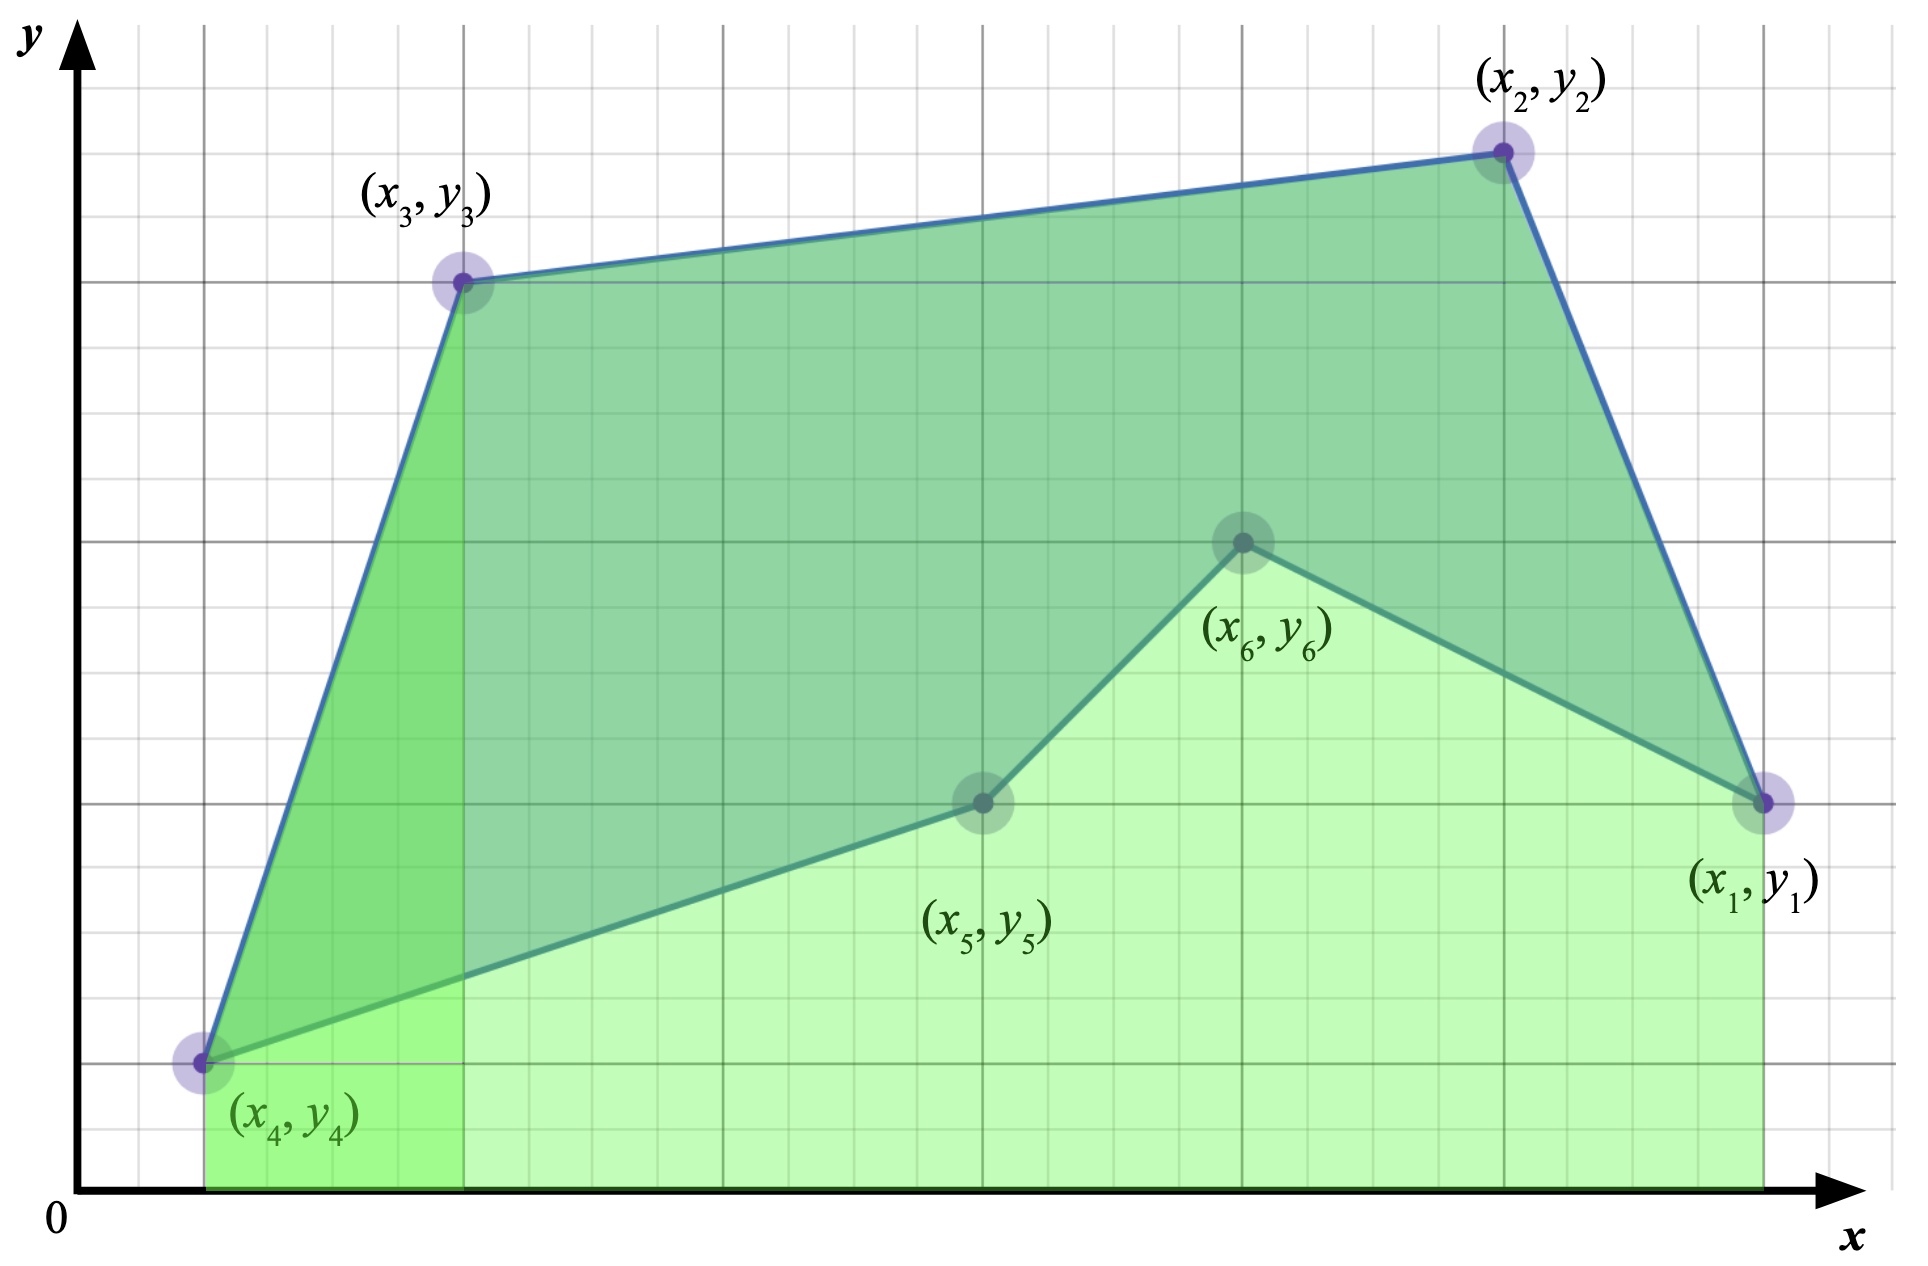
\includegraphics[width=0.8\linewidth]{media/shoelace/3-shoelace.png}
    \label{fig:shoe-3}
\end{figure}
\newpage
Note that a slightly darker green colour is used to indicate the last calculated trapezoid while a lighter green colour indicates an area that has already been calculated. The sum of the areas of the green regions from figure \ref{fig:shoe-3} is expressed mathematically, below.
\begin{align*}
    \text{Area of green region} &= 
    (\frac{1}{2}(y_1+y_2)(x_1-x_2))
    +(\frac{1}{2}(y_2+y_3)(x_2-x_3))
    +(\frac{1}{2}(y_3+y_4)(x_3-x_4))\\
    &=\frac{1}{2}((y_1+y_2)(x_1-x_2)
    +(y_2+y_3)(x_2-x_3)
    +(y_3+y_4)(x_3-x_4))
\end{align*}
Since $x,y\in\mathbb{R}^+$ and $x_1>x_2>x_3>x_4$, area of the green region a positive value.\newline

To remove the excess area within the green region to find the area of the shape from figure \ref{fig:shoe-0}, the trapezoid formula from equation \ref{eqn:trapezoid} is used again, since the area between the shape and the $x$-axis is also made up of trapezoids, as shown in the figures below.\newline

\begin{figure}[H]
    \centering
    \caption{Area of the first trapezoid of the excess area}
    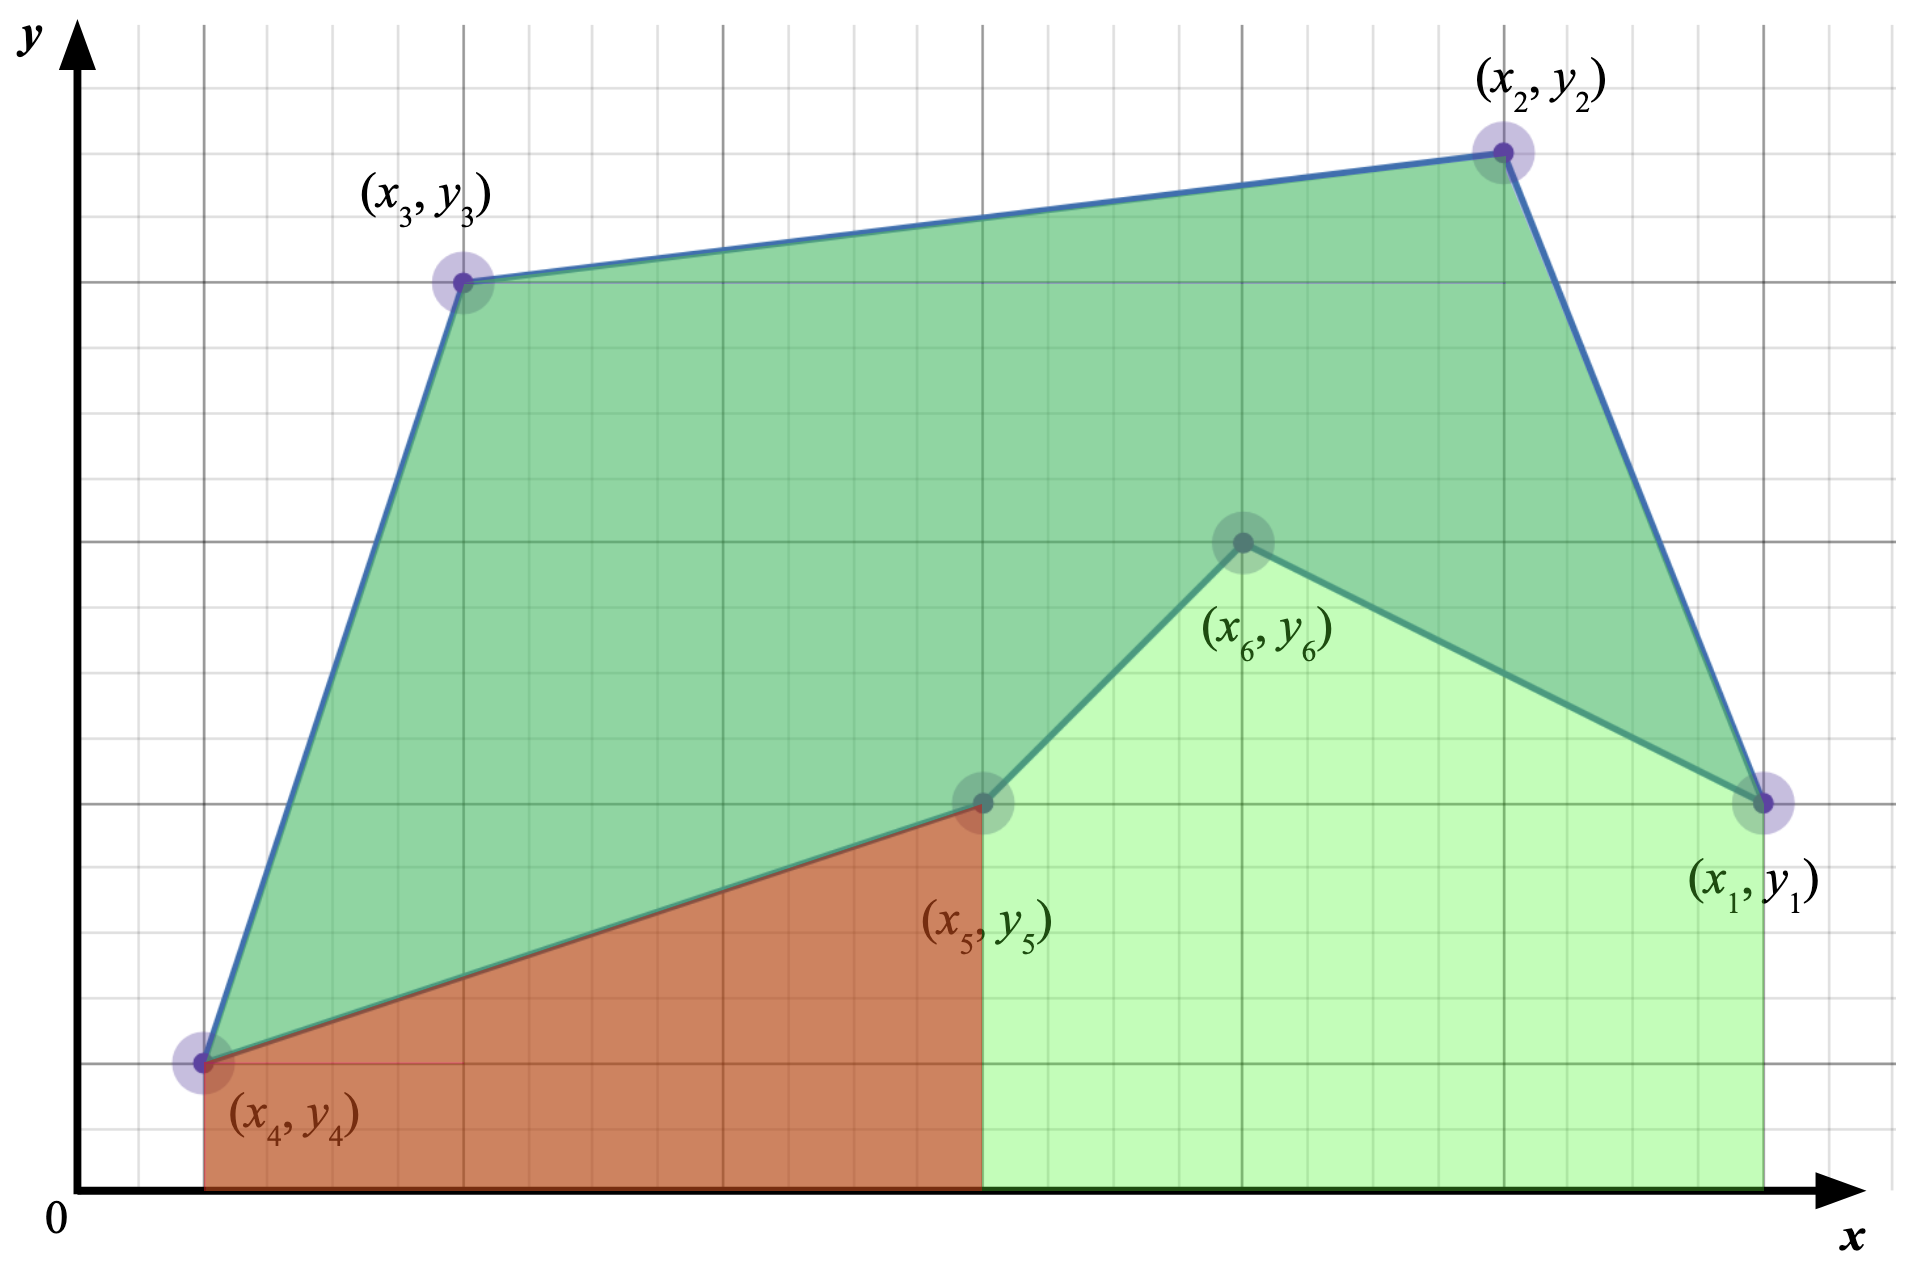
\includegraphics[width=0.8\linewidth]{media/shoelace/4-shoelace.png}
    \label{fig:shoe-4}
\end{figure}

In figure \ref{fig:shoe-4}, as well as the following two figures, the area of the red region is calculated as a negative value:
\bgroup
\allowdisplaybreaks
\begin{align*}
    \text{Recall from equation \ref{eqn:trapezoid}, }A&=\frac{1}{2}(a+b)h\\
    a&=y_4\\
    b&=y_5\\
    h&=x_4-x_5\\
    \therefore \text{Area of red region in figure \ref{fig:shoe-4}}&=\frac{1}{2}(y_4+y_5)(x_4-x_5)
\end{align*}
\egroup
$\frac{1}{2}(y_4+y_5)(x_4-x_5)$ is a negative value as $x_4<x_5$. And, by repeating the process for the next two trapezoids in figures \ref{fig:shoe-5} and \ref{fig:shoe-6} and adding up the areas, I would be able to obtain the negative value of the excess area between the shape and the $x$-axis.

\begin{figure}[H]
    \centering
    \caption{Area of the second trapezoid of the excess area}
    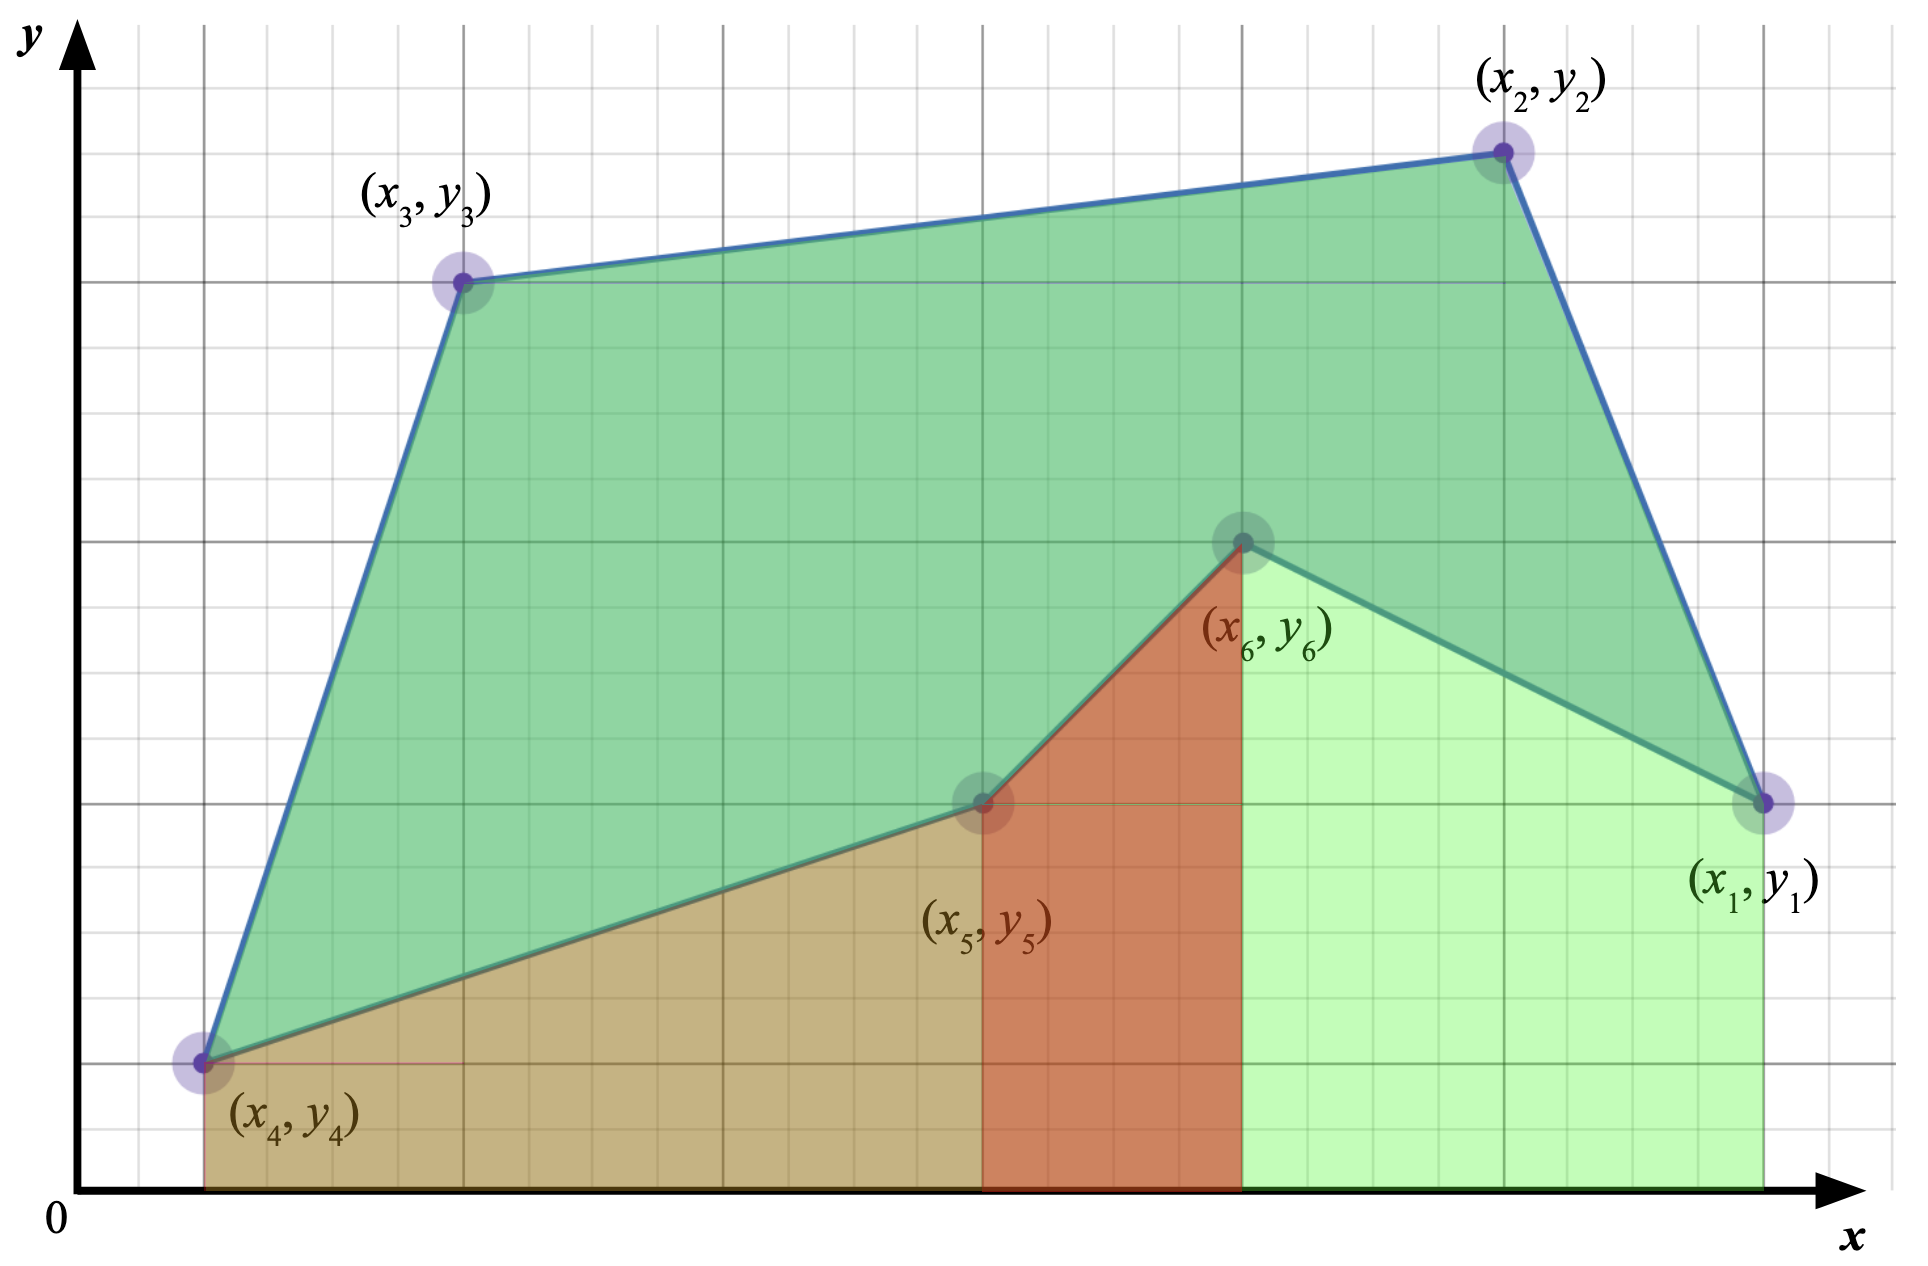
\includegraphics[width=0.8\linewidth]{media/shoelace/5-shoelace.png}
    \label{fig:shoe-5}
\end{figure}

\begin{figure}[H]
    \centering
    \caption{Area of the third trapezoid of the excess area}
    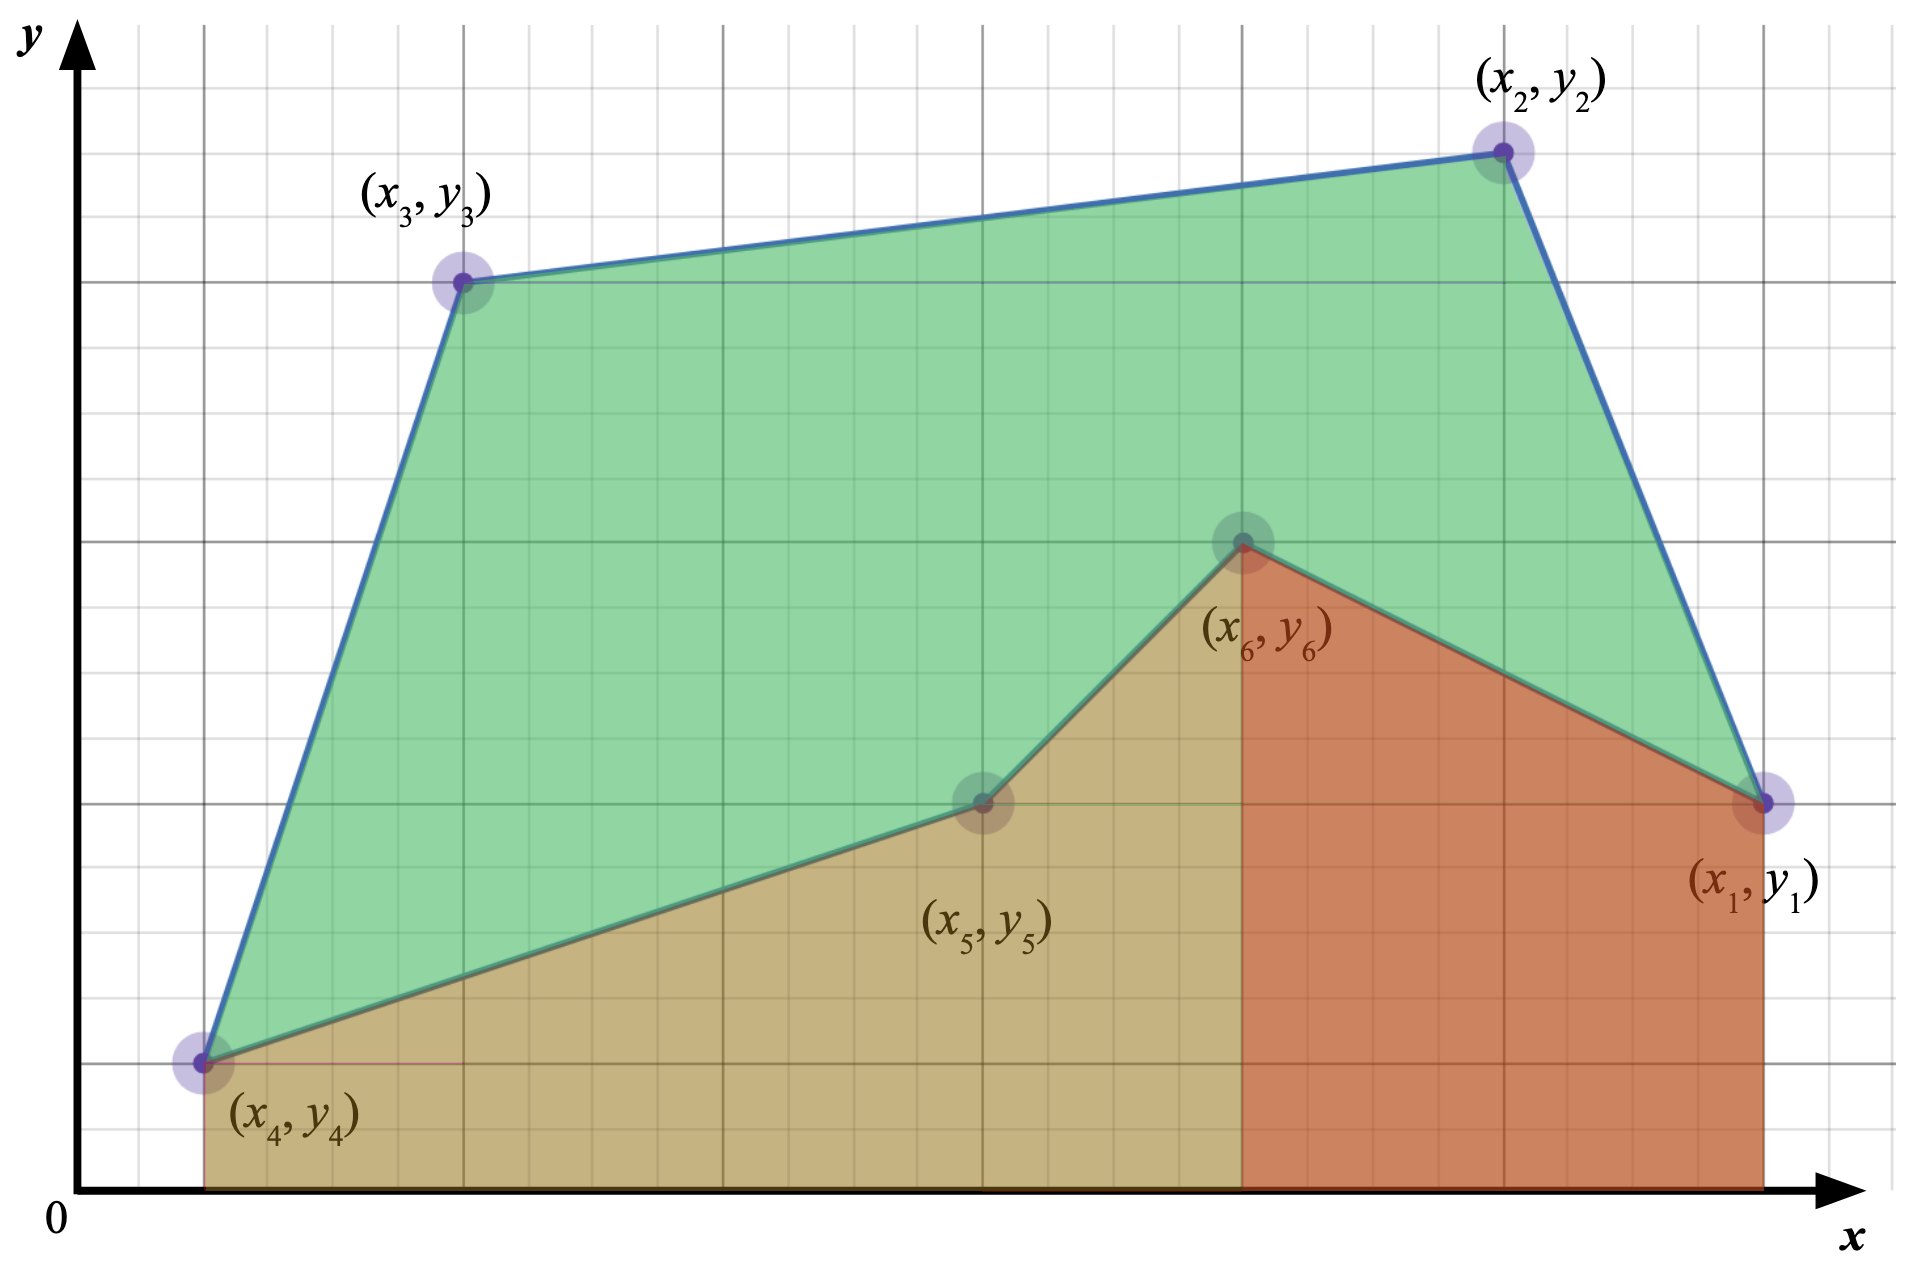
\includegraphics[width=0.8\linewidth]{media/shoelace/6-shoelace.png}
    \label{fig:shoe-6}
\end{figure}

Note that a red region indicates the portion of excess area that is being calculated and a brown region indicates that the portion of the excess area has already been calculated, with respect to the figure it is in.\newline

So, with the excess area being represented as the brown region in figure \ref{fig:shoe-7},
\begin{align*}
    \text{Excess area} &= 
    (\frac{1}{2}(y_4+y_5)(x_4-x_5))
    +(\frac{1}{2}(y_5+y_6)(x_5-x_6))
    +(\frac{1}{2}(y_6+y_1)(x_6-x_1))
    \\
    &=\frac{1}{2}((y_4+y_5)(x_4-x_5)
    +(y_5+y_6)(x_5-x_6)
    +(y_6+y_1)(x_6-x_1))
\end{align*}

\begin{figure}[H]
    \centering
    \caption{Result of the shoelace method for the example shape from figure \ref{fig:shoe-0}}
    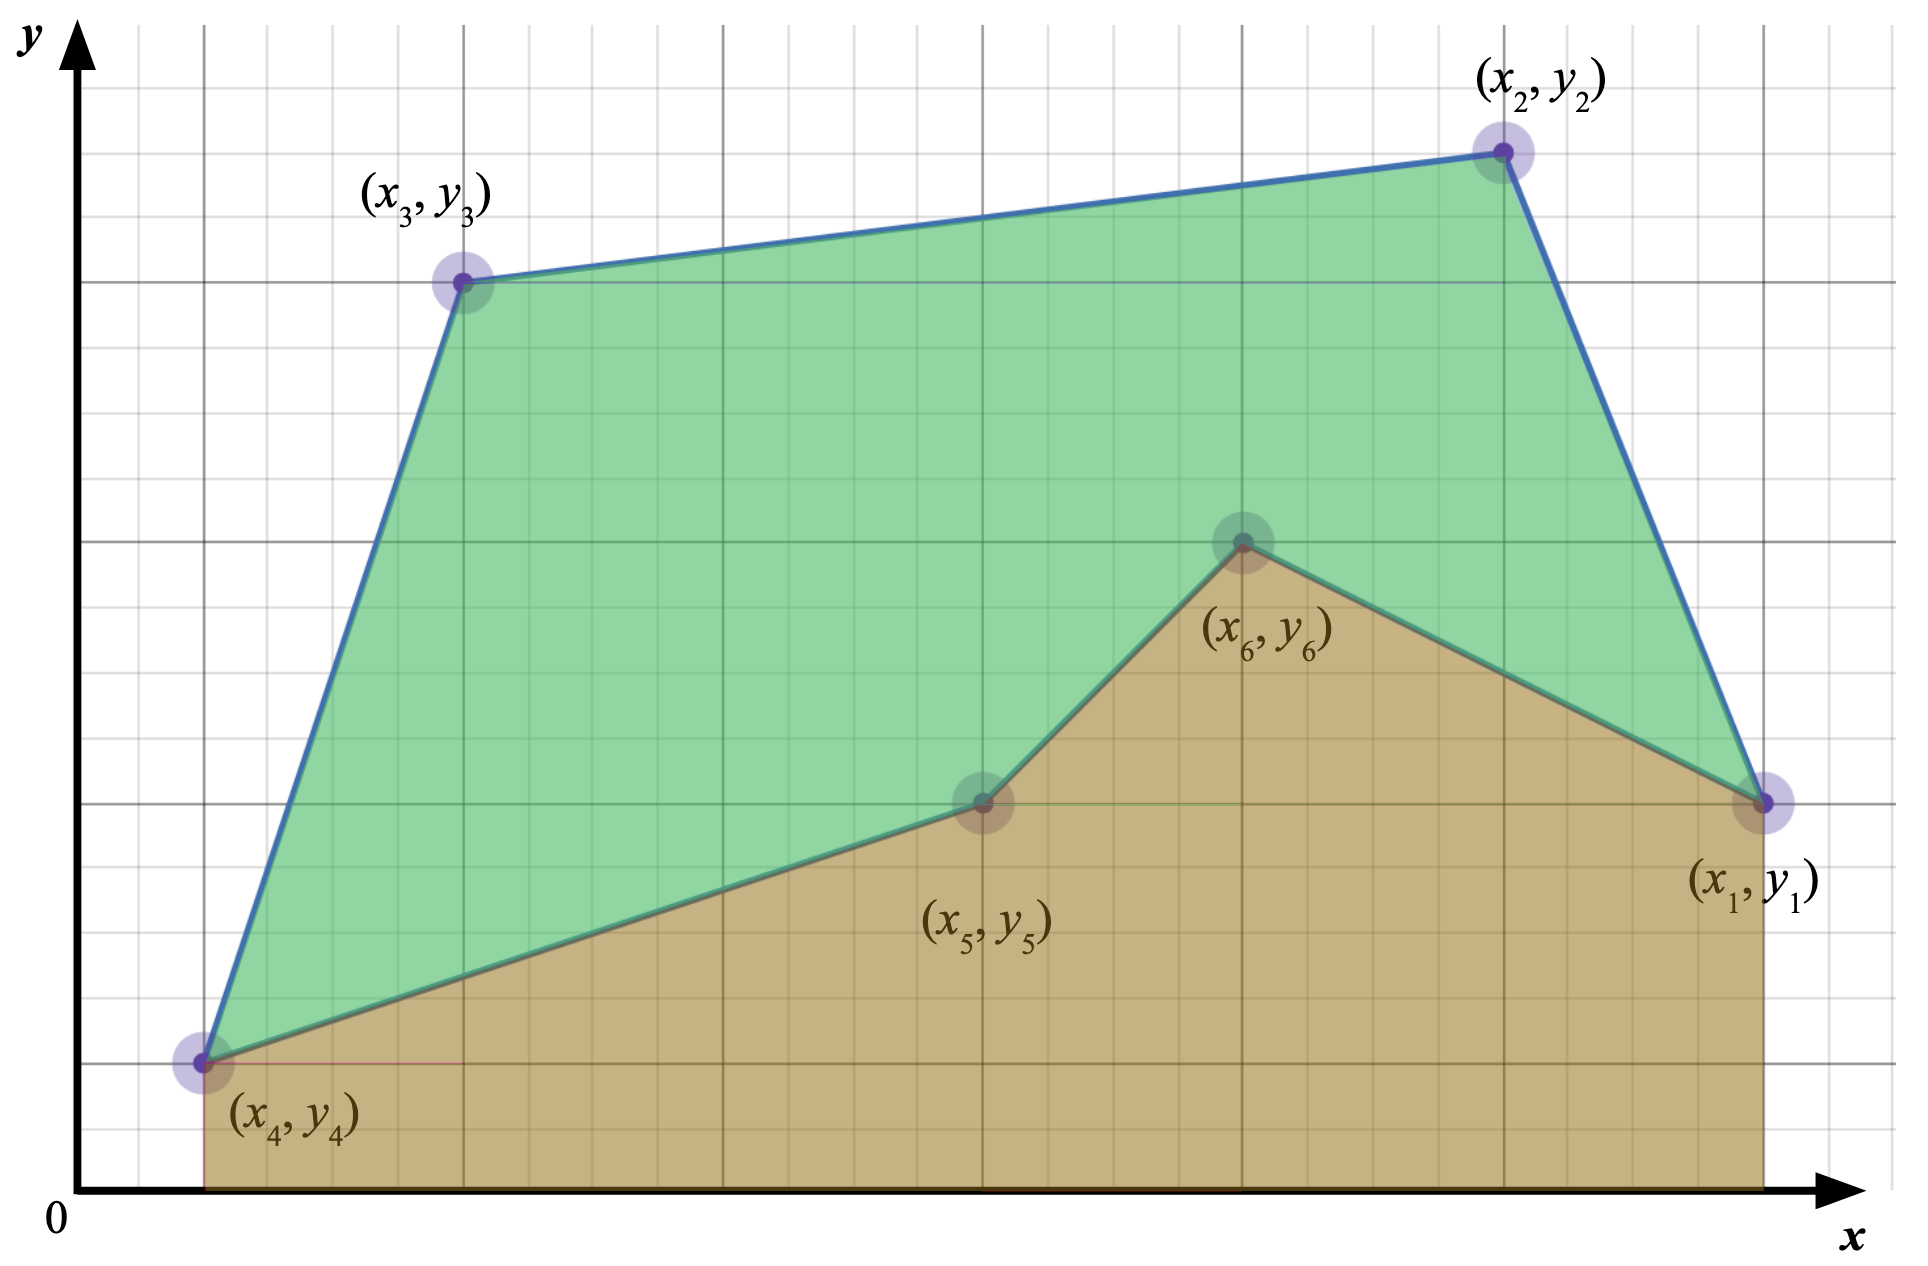
\includegraphics[width=0.8\linewidth]{media/shoelace/7-shoelace.png}
    \label{fig:shoe-7}
\end{figure}

Since the value of the excess area is negative due to $x_4<x_5<x_6<x_1$, I can simply add the excess area to the area of the green region in figure \ref{fig:shoe-3} to obtain the area of the shape in figure \ref{fig:shoe-0}. This is the same as subtracting the positive value of the area of the excess region from the positive value of the area of the green region. In the end, I would still be left with a remaining green region which would be the area of the shape, as shown in figure \ref{fig:shoe-7}.\newline

Notice that, in this example, the coordinates are arranged in an anti-clockwise orientation with the area of the green trapezoids being calculated from right to left before calculations of the area of the red trapezoids from left to right. Because of this, the value of the area of the shape is positive. If I were to have calculated the area with coordinates in a clockwise orientation, with the areas of the red trapezoids being calculated as positive values and the area of the green trapezoids calculated as negative values, the remaining area would be the negative value of the area of the shape from figure \ref{fig:shoe-0}. This explains why the formula for finding the area of an $n$-sided polygon using the shoelace method, as mentioned in equation \ref{eqn:shoelace-og}, has its $x$ and $y$ values enclosed in a absolute function; it will produce the same result for coordinates in a clockwise or anticlockwise orientation.\newline

So, the area of the six-sided polygon from figure \ref{fig:shoe-0} can be expressed as:
\bgroup
\singlespacing
\begin{align*}
    \text{Area} &=\text{Area of green region from figure \ref{fig:shoe-3} + Excess area}\\
    &=\frac{1}{2}((y_1+y_2)(x_1-x_2)
    +(y_2+y_3)(x_2-x_3)
    +(y_3+y_4)(x_3-x_4))\\&\qquad+
    \frac{1}{2}((y_4+y_5)(x_4-x_5)
    +(y_5+y_6)(x_5-x_6)
    +(y_6+y_1)(x_6-x_1))\\
    &=\frac{1}{2}((y_1+y_2)(x_1-x_2)
    +(y_2+y_3)(x_2-x_3)
    +(y_3+y_4)(x_3-x_4)\\&\qquad+
    (y_4+y_5)(x_4-x_5)
    +(y_5+y_6)(x_5-x_6)
    +(y_6+y_1)(x_6-x_1))
\end{align*}
\egroup

In fact, the equation above will provide the area of any six-sided polygon, given the coordinates of the polygon's corners in an anti-clockwise orientation.\newline

By generalising the working above such that the $6$th coordinate is now the $n$th coordinate and applying an absolute function to it, equation \ref{eqn:shoelace-og} can be derived for coordinates in an anti-clockwise or clockwise orientation:

\bgroup
\allowdisplaybreaks
\singlespacing
\begin{align*}
    \text{A}&=|\frac{1}{2}((x_1-x_2)(y_1+y_2)+(x_2-x_3)(y_2+y_3)+(x_3-x_4)(y_3+y_4)+\\
    &\qquad\dots\\
    &\qquad+(x_{n-2}-x_{n-1})(y_{n-2}+y_{n-1})+(x_{n-1}-x_{n})(y_{n-1}+y_{n})+(x_n-x_1)(y_n+y_1))|\\
    &=|\frac{1}{2}((x_1y_1-x_2y_2+x_1y_2-x_2y_1)\\
    &\qquad+(x_2y_2-x_3y_3+x_2y_3-x_3y_2)\\
    &\qquad+(x_3y_3-x_4y_4+x_3y_4-x_4y_3)+\\
    &\qquad\vdots\\
    &\qquad+(x_{n-2}y_{n-2}-x_{n-1}y_{n-1}+x_{n-2}y_{n-1}-x_{n-1}y_{n-2})\\
    &\qquad+(x_{n-1}y_{n-1}-x_ny_n+x_{n-1}y_n-x_ny_{n-1})+\\
    &\qquad+(x_ny_n-x_1y_1+x_ny_1-x_1y_n))|\\
    &=|\frac{1}{2}((x_1y_2-x_2y_1)+(x_2y_3-x_3y_2)+(x_3y_4-x_4y_3)+\\
    &\qquad\vdots\\
    &\qquad+(x_{n-2}y_{n-1}-x_{n-1}y_{n-2})+(x_{n-1}y_n-x_ny_{n-1})+(x_ny_1-x_1y_n))|\\
    \intertext{By grouping positive and negative $xy$ values together,}
    \text{A}&=|\frac{1}{2}(x_1y_2 + x_2y_3 + x_3y_4 + \dots + x_{n-2}y_{n-1} + x_{n-1}y_n + x_ny_1\\ 
    &\qquad- x_2y_1 - x_3y_2 - x_4y_3 - \dots - x_{n-1}y_{n-2} - x_ny_{n-1} - x_1y_n)|\\
    &=\frac{1}{2}|(x_1y_2 + x_2y_3 + x_3y_4 + \dots + x_{n-2}y_{n-1} + x_{n-1}y_n + x_ny_1)\\
    &\qquad-(x_2y_1 + x_3y_2 + x_4y_3 + \dots + x_{n-1}y_{n-2} + x_ny_{n-1} + x_1y_n)|\qquad QED
\end{align*}
\egroup

The shoelace method is shown to be a sum of the positive and negative areas of trapezoids with the use of its coordinates in an anti-clockwise or clockwise orientation.\newline

Using this knowledge, I decided to represent the AOS as a 42-sided polygon, with the 42 coordinates it as made up of shown in the figure below.

\begin{figure}[H]
    \centering
    \caption{Coordinates of corners of the AOS polygon}
    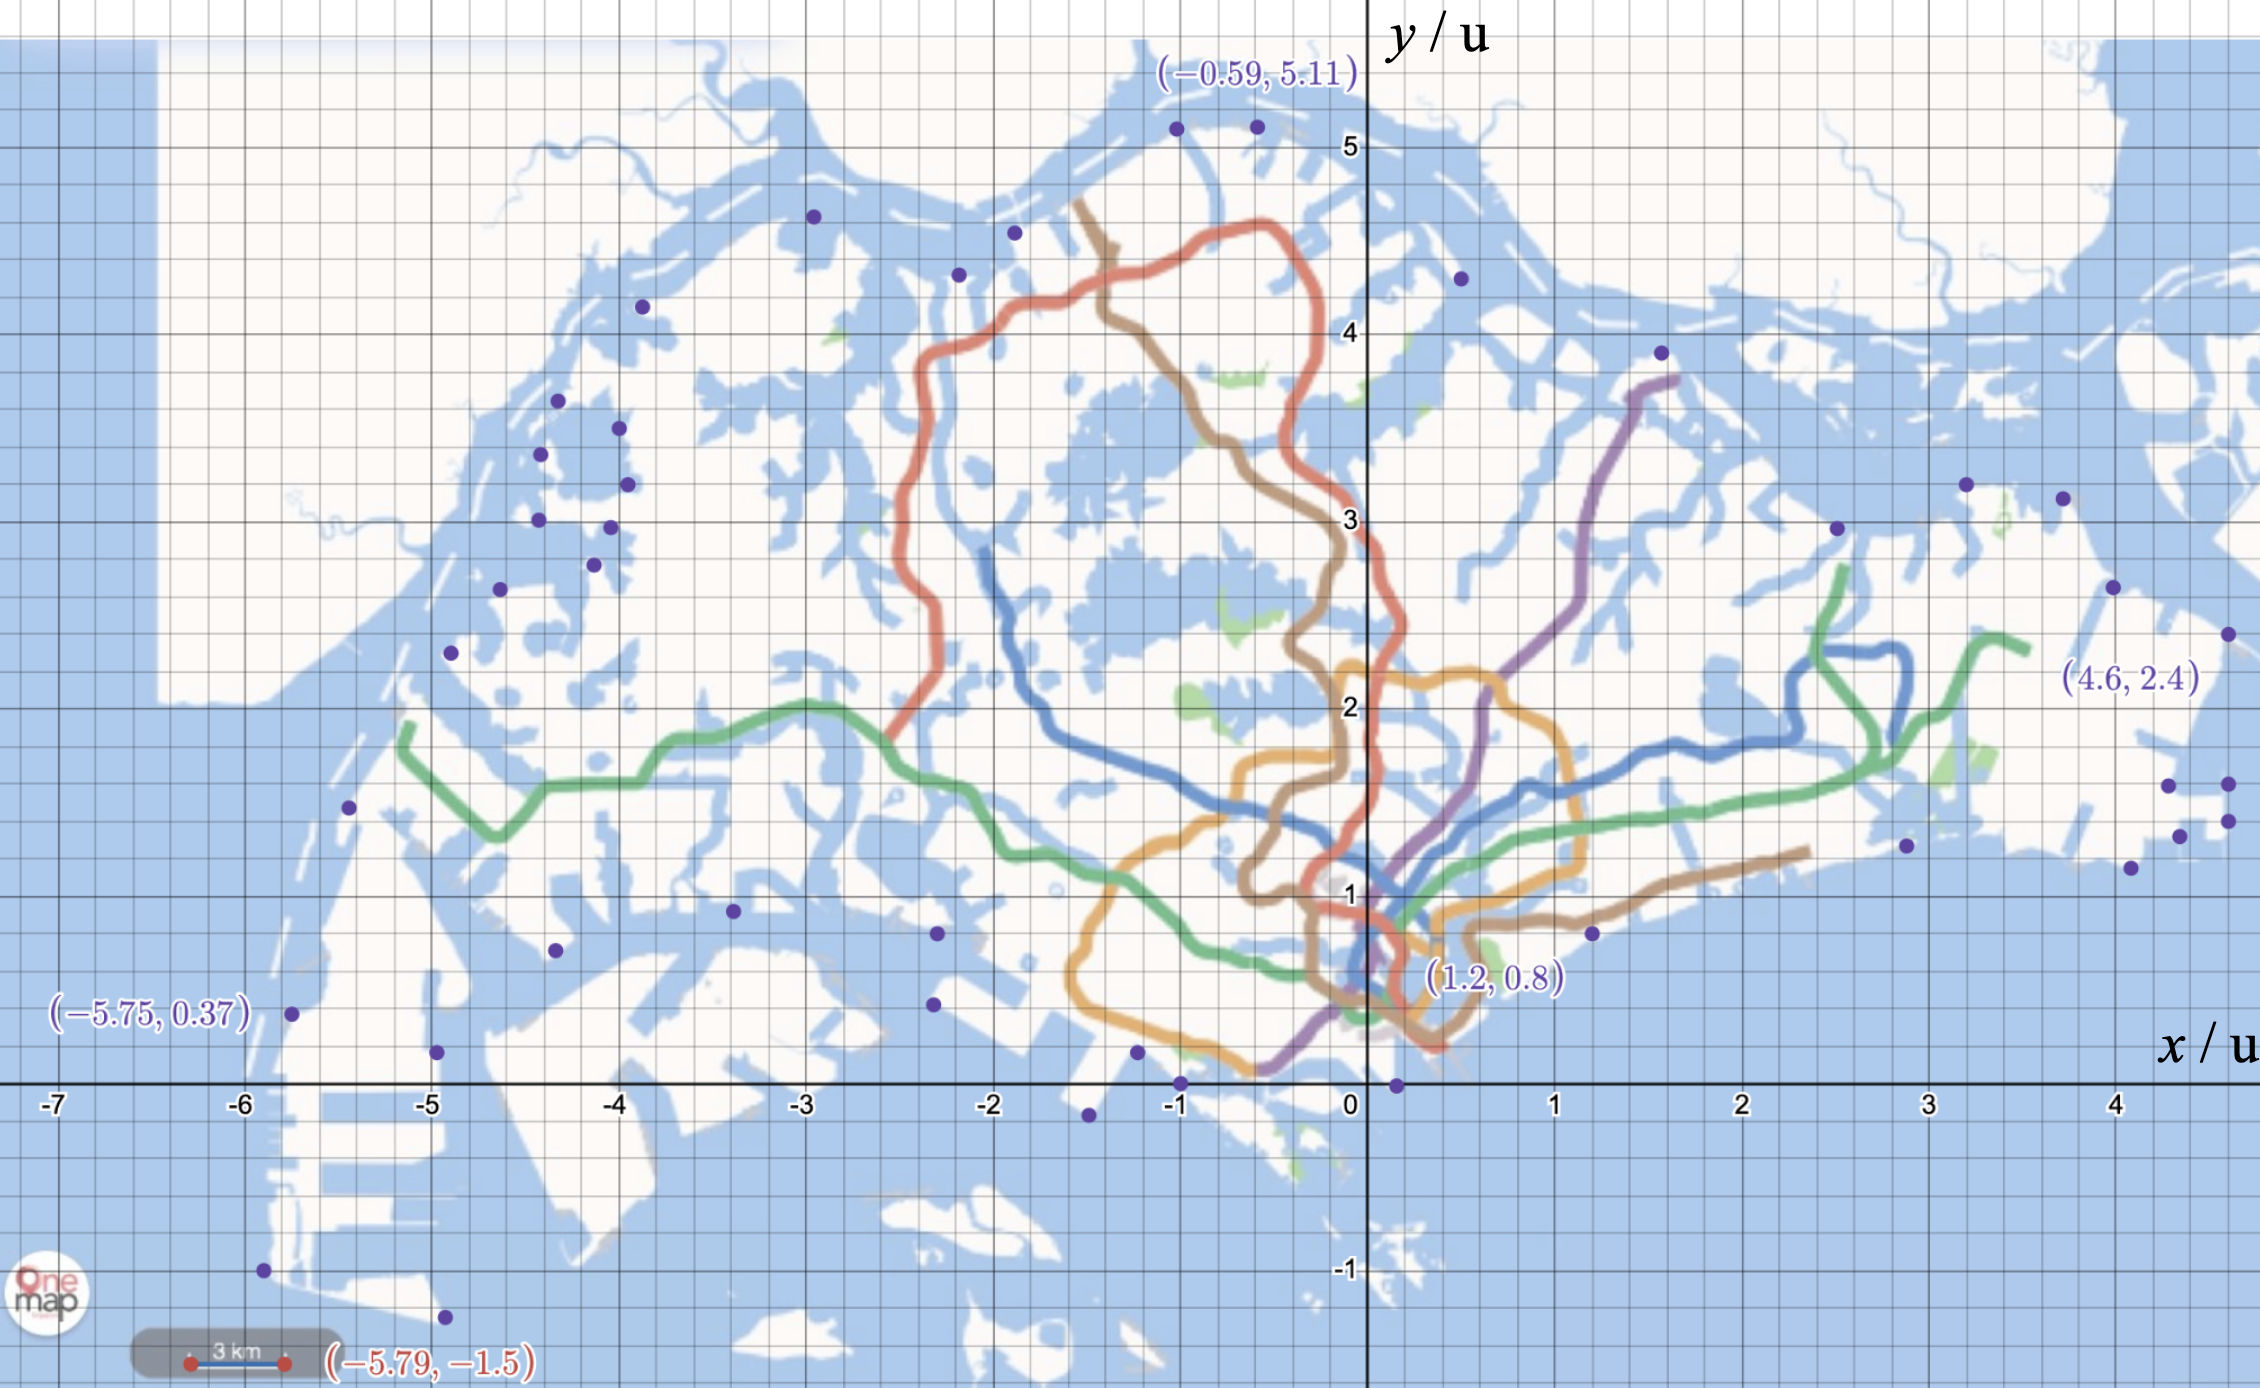
\includegraphics[width=0.7\linewidth]{media/shoelace-units.png}
    \label{fig:coords}
\end{figure}

In figure \ref{fig:coords}, for reference and readers’ convenience, the first, thirteenth, twentieth and twenty seventh coordinate are labelled in purple, with an anticlockwise orientation. The values of the $x$ and $y$ coordinates of the $i$-th coordinate out of a total of 42 coordinates that were plotted are shown in appendix \ref{appendix:shoe-coords}. To calculate the AOS using the shoelace formula from equation \ref{eqn:shoelace-og}, I utilised Google Sheets to automatically calculate the areas, with the calculated values found in appendix \ref{appendix:shoe-vals}.\newline

From equation \ref{eqn:shoelace-og}, $\text{AOS }= \frac{1}{2}|(x_1y_2+x_2y_3+\dots+x_{42}y_1)-(x_2y_1+x_3y_2+\dots+x_1y_{42})|$. So, if

\vspace*{-8mm}
\bgroup
\singlespacing
\allowdisplaybreaks
\begin{align*}
(x_1y_2+x_2y_3+\dots+x_{42}y_1)&=32.679848\text{ u}^2\\
\intertext{and}
(x_2y_1+x_3y_2+\dots+x_1y_{42})&=-0.281979\text{ u}^2\\
\intertext{then} \text{AOS}
    &=32.679848\text{ u}^2-(-0.281979)\text{ u}^2\\
    &=32.679848\text{ u}^2+0.281979\text{ u}^2\\
    &=32.961827 \text{ u}^2\\
    &=36\times 32.961827 \text{ km}^2\\
    &=1186.625772 \text{ km}^2\\
    &\approx 1190 \text{ km}^2
\end{align*}
\egroup

While the new approximation of the AOS of $1190 \text{ km}^2$ is more precise than the previous approximation that was made through the use of simple geometric shapes, I realised that one significant limitation of the Shoelace method was its lack of precision around curved edges of a shape due to its nature of utilising coordinates. Therefore, I decided to utilise integration with quadratic curves to find a more accurate AOS.\newline

Figure \ref{fig:curves-sketch} is a rough sketch of the curved coastline of Singapore, indicated by the u-shaped lines that are drawn. The map of Singapore is shown in black and white so that the lines can be seen better. It is my intention to integrate each quadratic curve to find the areas under them, which would overlap the AOS. In order to do so, the extra area below the Singapore island would need to be subtracted. This is indicated by the different coloured lines, where an area under the red curves are subtracted from the sum of an area under each of the green curves to calculate the value of the AOS.

\begin{figure}[H]
    \centering
    \caption{Sketch of curved edges of Singapore's coastline}
    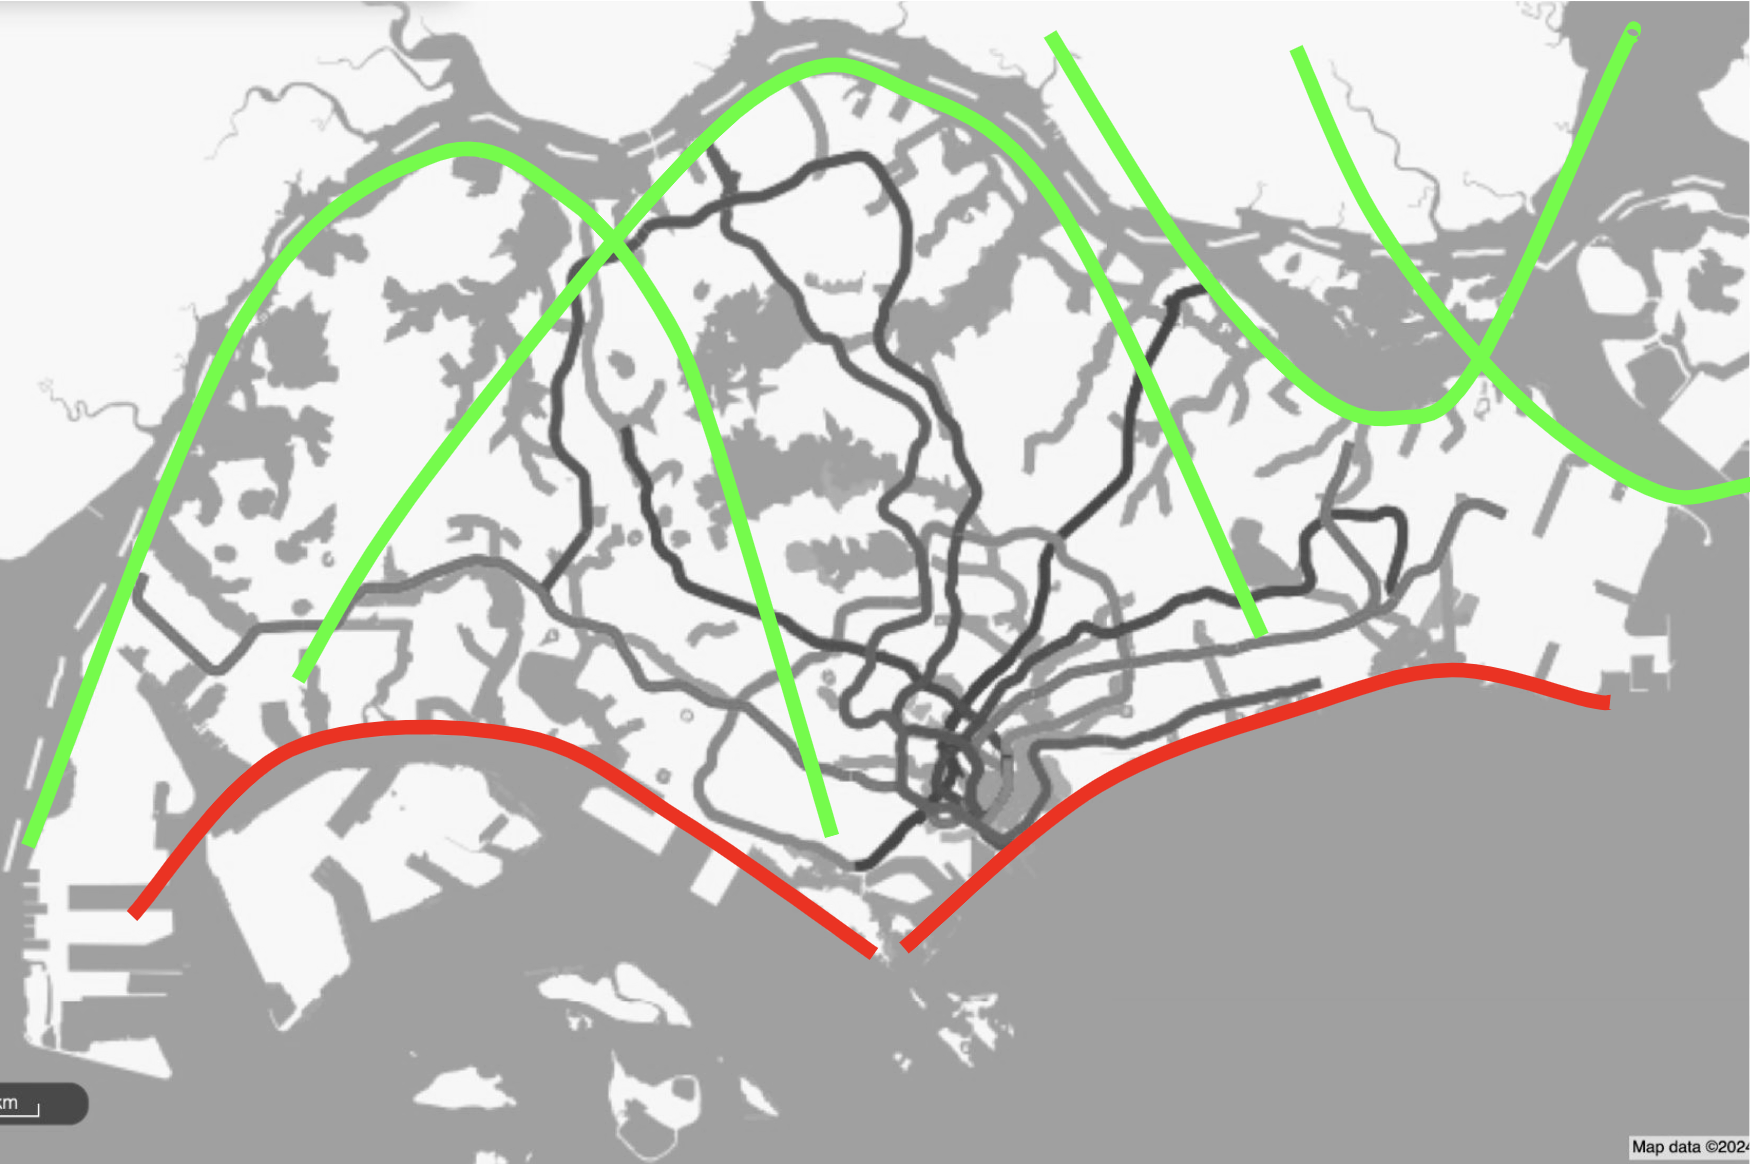
\includegraphics[width=0.8\linewidth]{media/curves-sketch.png}
    \label{fig:curves-sketch}
\end{figure}

Since the sketched curves in figure \ref{fig:curves-sketch} seems to resemble different quadratic curves, I utilised Desmos to form the six quadratic equations that resembles the different sketched curves by plotting quadratic regression curves with exactly three coordinates for each of the six quadratic equations.\newline

While the three coordinates are unanimously adjusted to translate a given quadratic curve along the $x$ or $y$ axis to outline parts of the coastline of Singapore, the reason behind the use of exactly three coordinates per quadratic curve is because, out of the three coordinates, the coordinate with the maximum or minimum $y$-coordinate value is positioned such that its $x$-coordinate value is exclusively between the other two $x$-coordinate values, allowing me to dictate the sign of the quadratic regression curve that would be plotted. Next, adjusting the $x$ and $y$ values of the other two coordinates would allow me to control the shape of the quadratic functions that would outline the Singapore coastline by stretching or contracting the quadratic curves along the $x$-axis.\newline

Throughout the entire graph transformation process, the three coordinates that are used for each quadratic curve would always lie somewhere along the curve; the $R^2$ value, which is a measurement of how well a regression model fits the data it is in relation to, of each quadratic curve plotted would always be equal to the best possible value of $1$, ensuring accuracy in the positioning of each quadratic curve in relation to the coordinates that are used \parencite{r_sqr_fccamp, r_sqr_investopedia}. The resulting quadratic functions are graphed in the figures below.\newline

\begin{figure}[H]
    \centering
    \caption{Quadratic curves along Singapore coastline}
    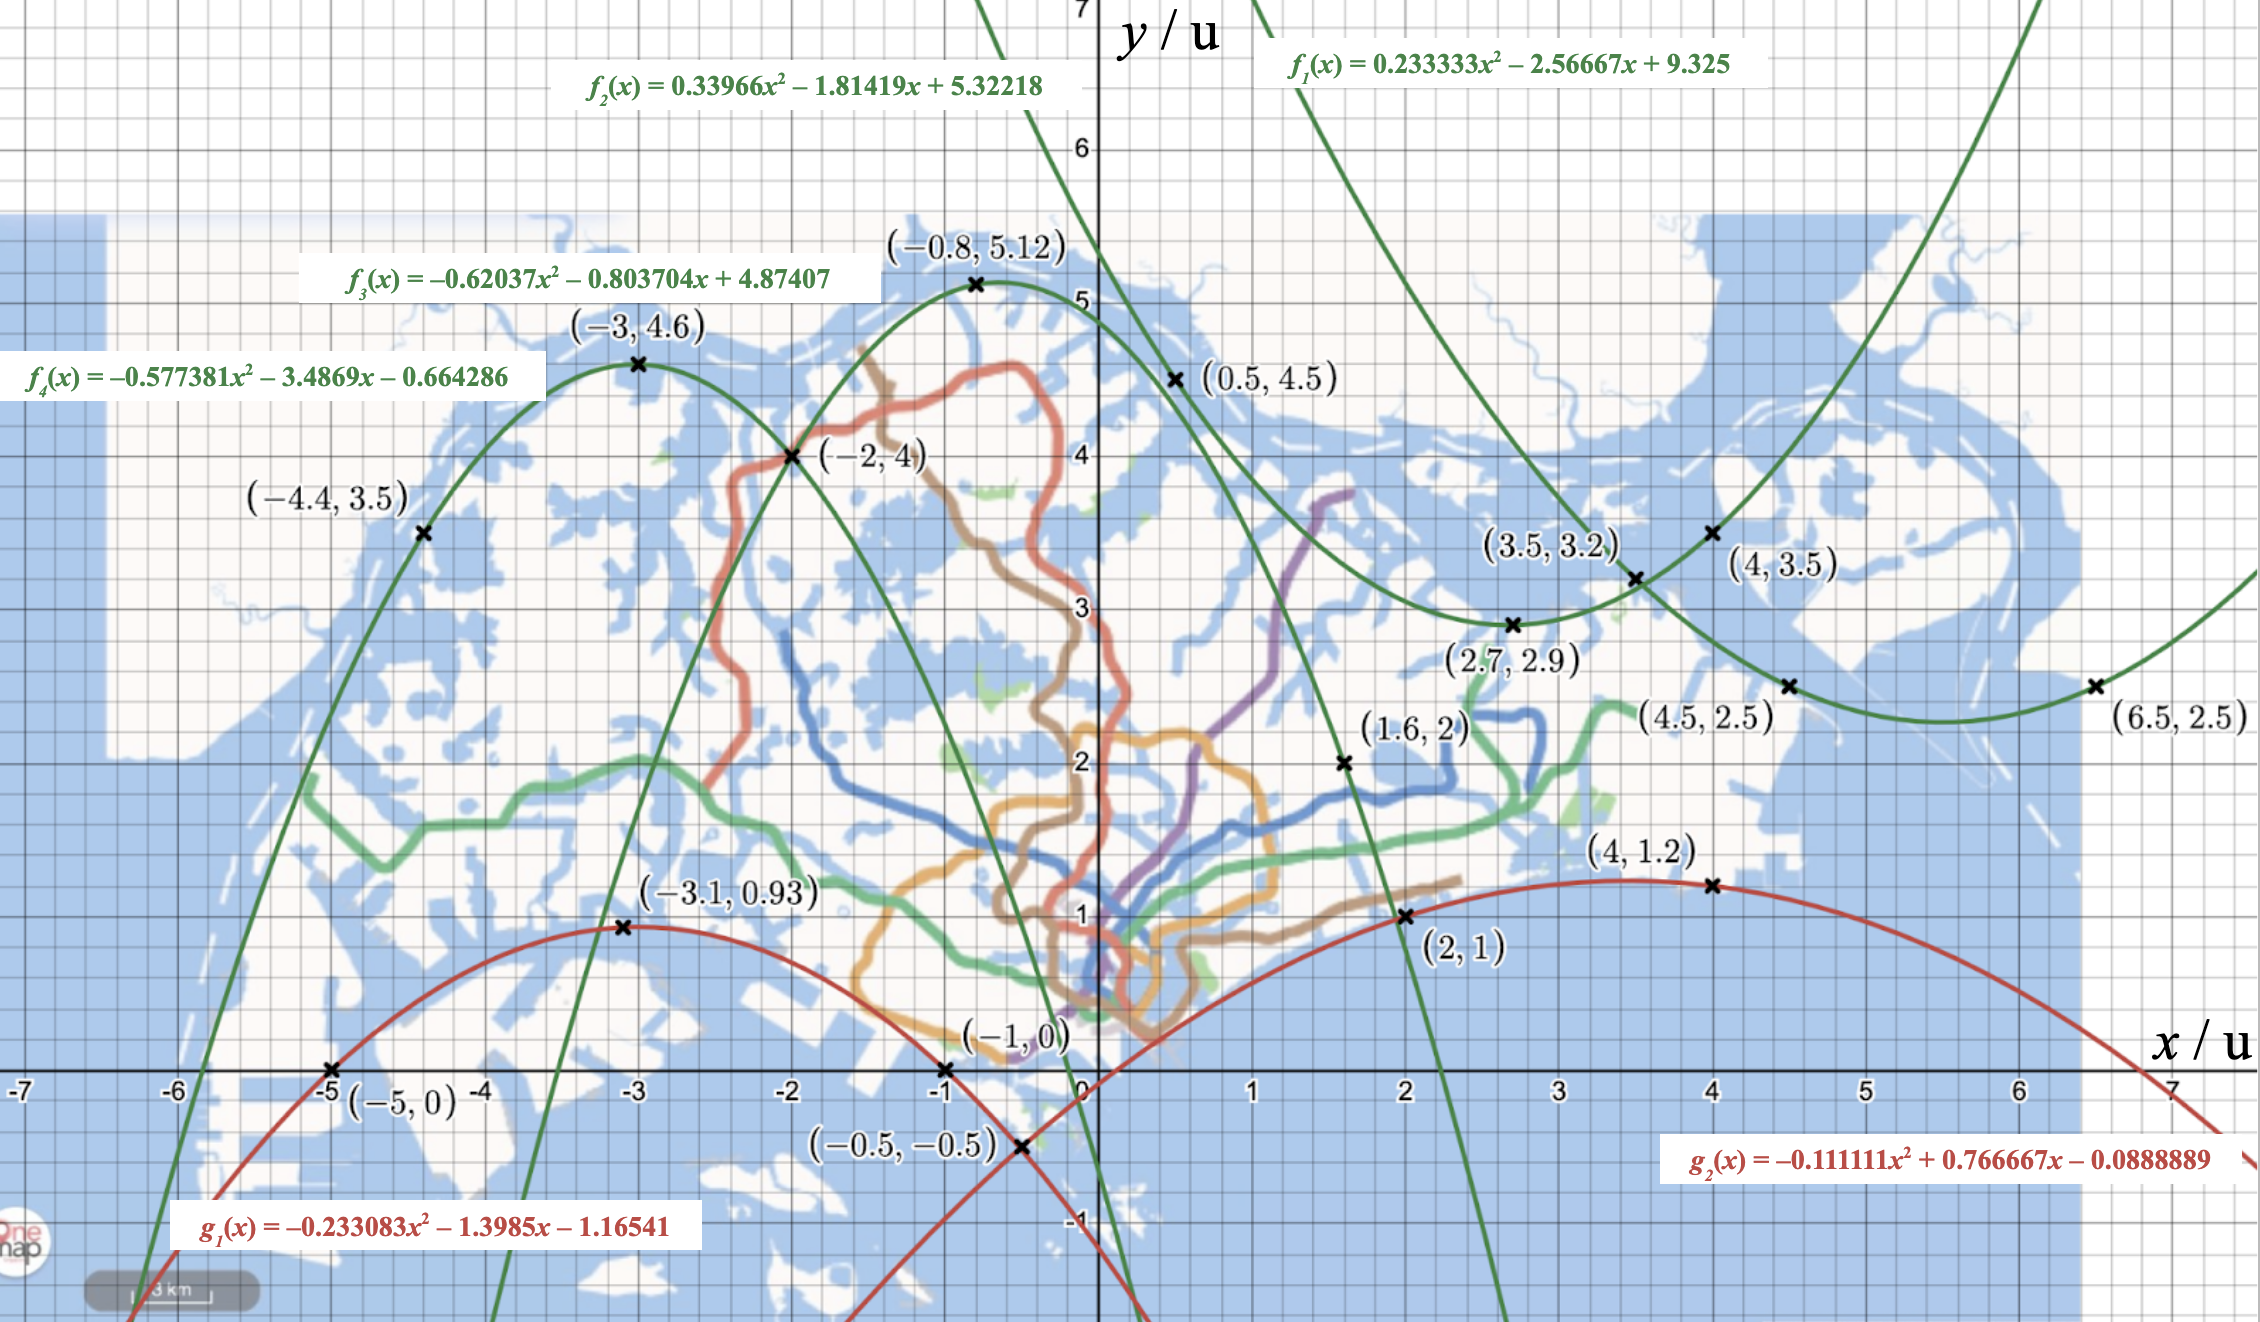
\includegraphics[width=0.9\linewidth]{media/int-labelled-units.png}
    \label{fig:int}
\end{figure}

In figure \ref{fig:int}, six quadratic curves are plotted such that a segment of the curve follows the general curvature of a part of the Singapore coastline. Each of the six curves intersect at least three coordinates, which were used to obtain the equations of said quadratic curves. Points of intersection between like-coloured curves are also marked. Since the AOS comprises only of certain segments of the area between the green and red graphs, the quadratic curves are split into segments in the diagram below.\newline

\begin{figure}[H]
    \centering
    \caption{Splitting the Singapore map into sectors for integration}
    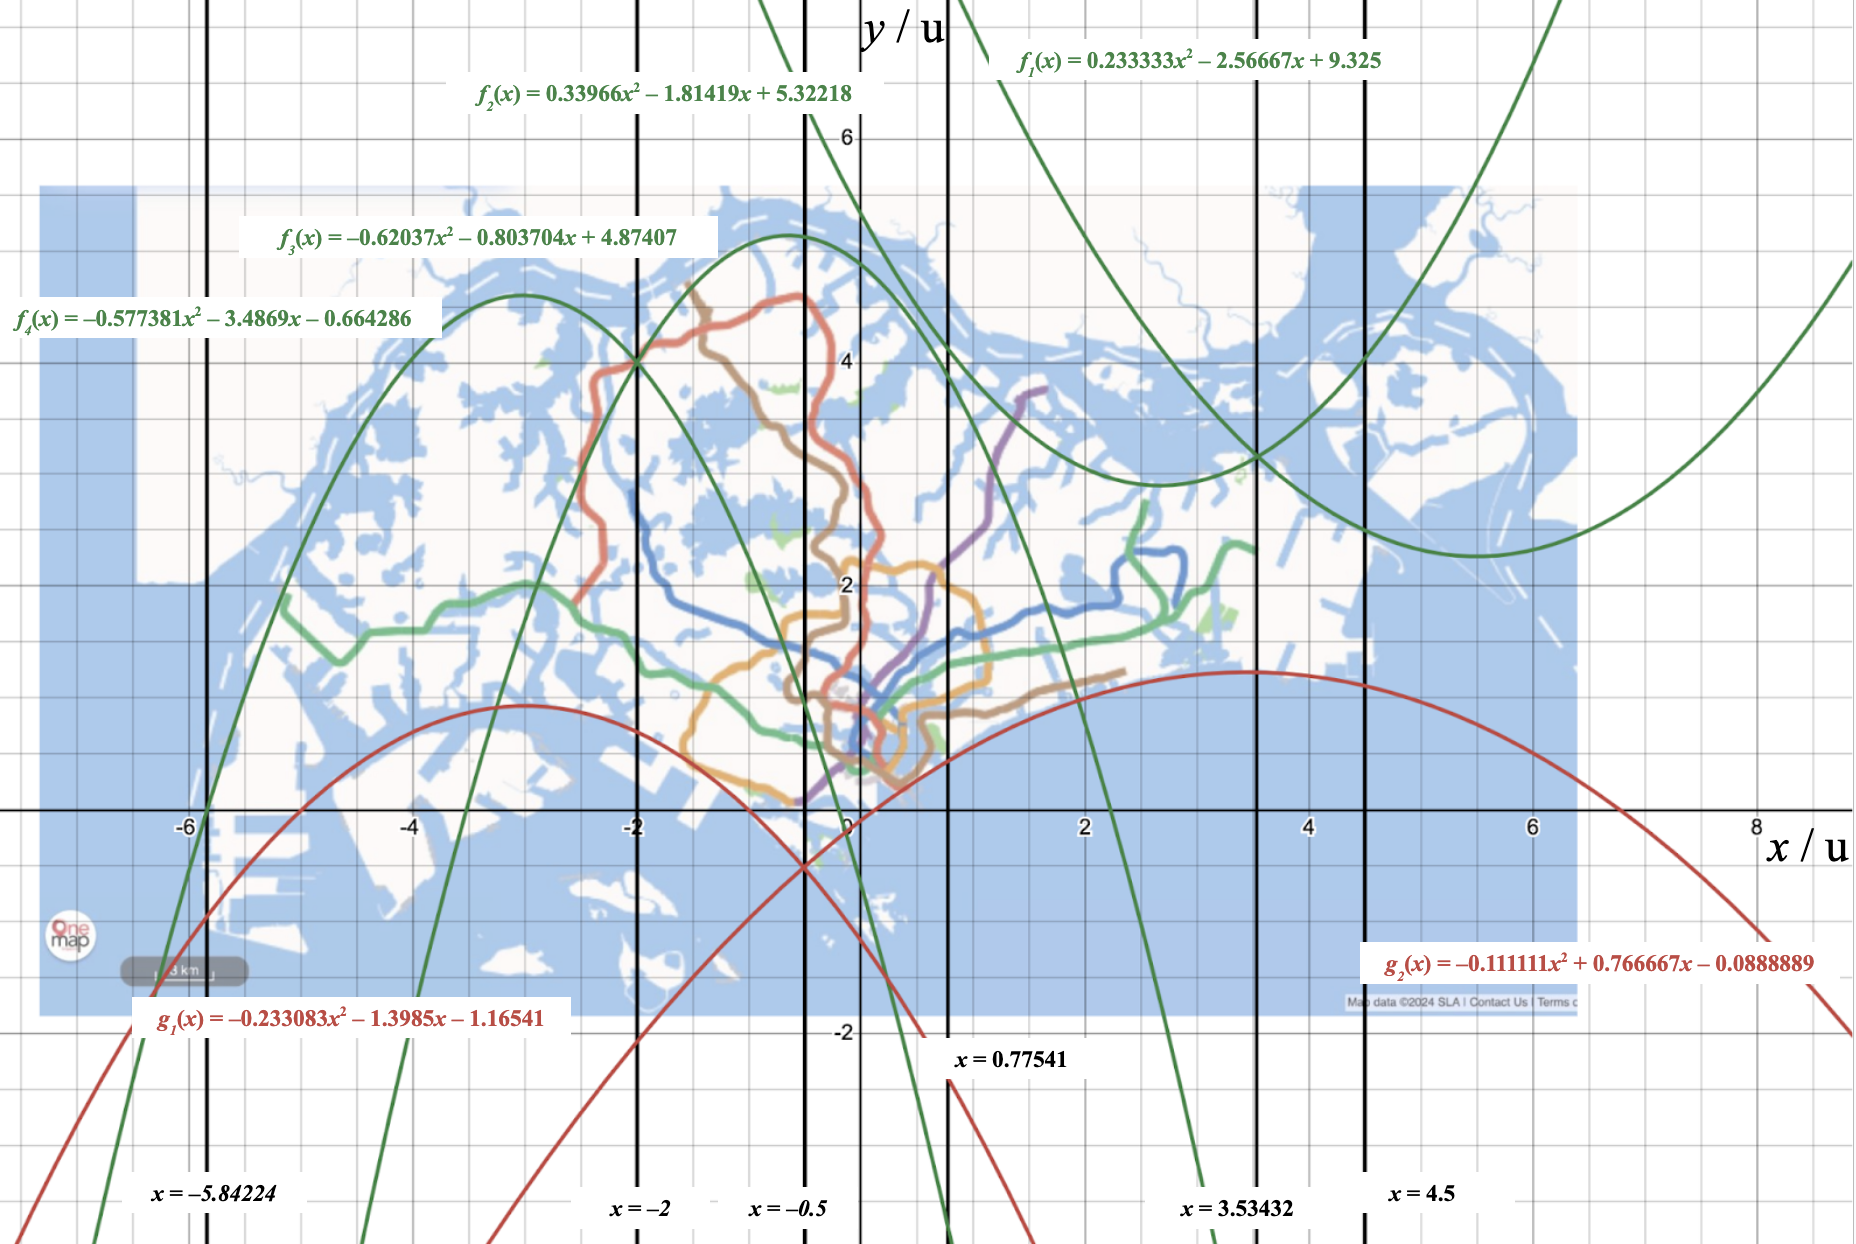
\includegraphics[width=0.9\linewidth]{media/int-sectors-units.png}
    \label{fig:int-sectors}
\end{figure}

In figure \ref{fig:int-sectors}, the map is split into segments based on the start and end of each quadratic curve. The black lines indicate the upper and lower bounds of the integrals of the quadratic curves so that only the area enclosed by one green, two black and one red lines would be accounted for.\newline

Figure \ref{fig:int-simple} shows a simplified version of the quadratic curves, where only the segments of the curve that  factor in to the calculation of the AOS are shown. Essentially, the area under the red segments will be subtracted from the area under the green segments, which would provide the AOS in terms of $\text{u}^2$.\newline

\begin{figure}[H]
    \centering
    \caption{Simplified view of using quadratic curves to find the AOS}
    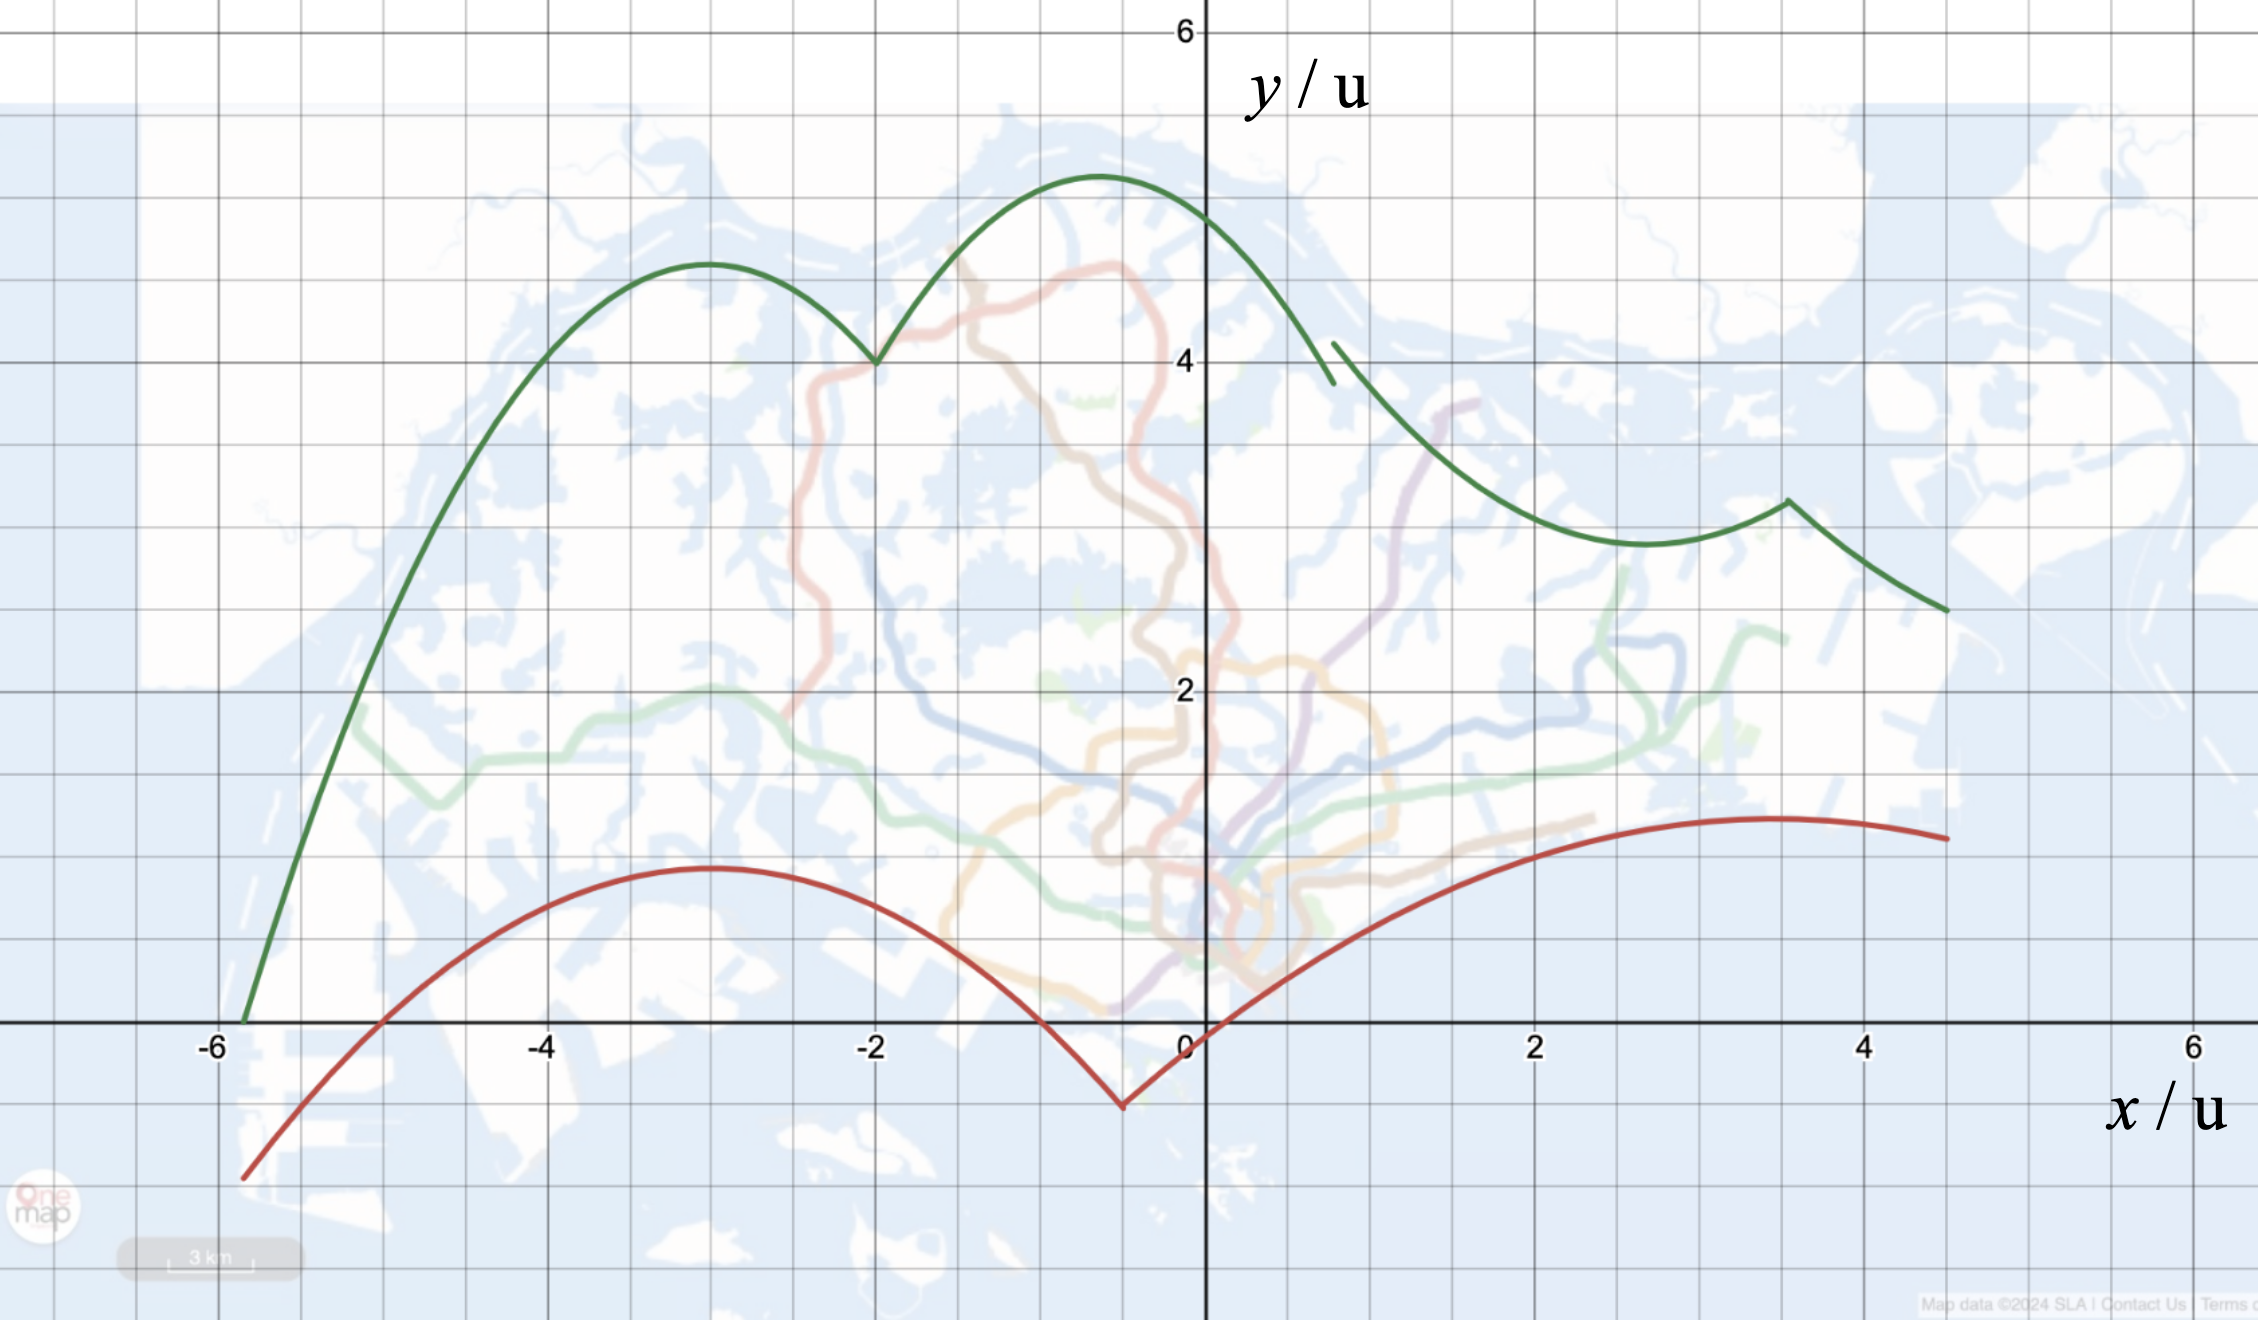
\includegraphics[width=0.9\linewidth]{media/integration-ez-units.png}
    \label{fig:int-simple}
\end{figure}

According to the \cite{ib}, $\int x^n\text{ }dx=\frac{x^{n+1}}{n+1}+C,\quad n\neq-1$. So,
\begin{align*}
    \text{if } y&=ax^2+bx+k,\quad a\neq-1 \text{, }b\neq-1\\
    \int^{\text{}}_{\text{}}y\text{ }dx&=\frac{a}{3}x^3+\frac{b}{2}x^2+kx+C\text{ },\quad C\in\mathbb{R}\\
    \therefore \int^h_ly\text{ }dx&=(\frac{a}{3}h^3+\frac{b}{2}h^2+kh)-(\frac{a}{3}l^3+\frac{b}{2}l^2+kl)\text{ }, \quad \forall h,l \in \mathbb{R}
\end{align*}

Because some segments of the quadratic curves are below the $x$-axis of $y=0$ as shown in figure \ref{fig:int-simple}, the formula for finding the area between curves with a given interval will be used. According to \cite{libretext},

\begin{equation}\label{eqn:int-formula}
    A=\int^u_p[f(x)-g(x)]\space dx,\quad f(x)\geq g(x),\space u<p
\end{equation}

In the equation above, $A$ represents the area between $f(x)$ and $g(x)$ with interval $u,p$.\newline

Using the black vertical lines drawn in figure \ref{fig:int-sectors} to obtain the intervals of integrals, equation \ref{eqn:int-formula} can be applied to find the AOS in u$^2$ by summing up the areas between the following curves:

\begin{itemize}
    \item $f_1(x)$ and $g_2(x)$ where $3.53432<x<4.5$
    \item $f_2(x)$ and $g_2(x)$ where $0.77541<x<3.53432$
    \item $f_3(x)$ and $g_2(x)$ where $-0.5<x<0.77541$
    \item $f_3(x)$ and $g_1(x)$ where $-2<x<-0.5$
    \item $f_4(x)$ and $g_1(x)$ where $-5.84224<x<-2$
\end{itemize}

Note that, since $f_3(x)$ is above the intersection of $g_1(x)$ and $g_2(x)$, the calculation of the area between the green quadratic curve of $f_3(x)$ and the red quadratic curves below it has to be done in two parts.\newline

The mathematical working for the approach above is shown in appendix \ref{appendix:int-maths}, where the differences between the green quadratic curves and the red quadratic curves are calculated first before their resulting values are integrated, with the use of equation \ref{eqn:int-formula}, and summed up. Since calculating the difference in the above quadratic functions was tedious, I utilised WolframAlpha to automatically calculate the differences between the green quadratic curves and the red quadratic curves.\newline

As a result, the AOS is $1152.13016\text{ km}^2\approx1150\text{ km}^2$ when calculated using the integrals of different quadratic functions and rounded to 3 significant figures. This value is consistent with the previously calculated values of $1050\text{ km}^2$ and $1190\text{ km}^2$, where $1050\text{ km}^2<\textbf{1150 km}^2<1190\text{ km}^2$. I was able to confirm my findings using Desmos's graphical calculator demonstrated in appendix \ref{appendix:int-confirm}, obtaining a value of $1152.19299881\text{ km}^2\approx1150\text{ km}^2$. While $1152.19299881\text{ km}^2\neq1152.13016\text{ km}^2$ due to the loss of decimal places when using WolframAlpha, the difference is insignificant given that both would equal $1150 \text{ km}^2$ when rounded to 3 significant figures. While the use of quadratic curves cannot accommodate sharp edges in the coastline as well as other methods in this investigation, I think that the use of integration to find the AOS is the most precise method as the majority of the quadratic functions drawn mimicked the coastline of Singapore accurately.\newline

According to the \cite{land_auth} and the \cite{dss}, the official land area of Singapore is $735.7$ km$^2$ as of December 2024, discounting the surface area of certain bodies of water based on geographic factors. As expected, my most accurate estimation of the AOS of $1150\text{ km}^2$ is greater than the official approximation of the land area of Singapore as my methodology includes all bodies of water that run through and within Singapore. I believe that the use of integration to find the AOS by summing up areas between different quadratic curves is not only the most accurate in the context of this investigation, but also the most practical as its accuracy is not as dependent on the number of Cartesian coordinates that are used, when compared to the previous methods involving basic geometrical shapes and the use of the Shoelace theorem. When using methods with an accuracy that is heavily reliant on the number of coordinates provided, plotting points and obtaining coordinates by hand can be very time consuming and poses risks of human error. Instead, methods involving geometry and the Shoelace theorem could be more applicable in a fully-automated system, such as a computer vision edge detection program, that is able to generate many more coordinates reliably \parencite{edge_detect}.

%TC:ignore
\newpage
\appendix
\appendixpage

\section{Coordinates used for the shoelace method}\label{appendix:shoe-coords}
\bgroup
\begin{table}[H]
\renewcommand\tabularxcolumn[1]{m{#1}}
\renewcommand{\arraystretch}{1}
\centering
\resizebox{0.6\textwidth}{!}{%
\footnotesize
\begin{tabular}{|r|r|r|l|r|r|r|}
\cline{1-3} \cline{5-7}
\multicolumn{1}{|l|}{\textbf{$i$}} & \multicolumn{1}{l|}{\textbf{$x_i$}} & \multicolumn{1}{l|}{\textbf{$y_i$}} &  & \multicolumn{1}{l|}{\textbf{$i$}} & \multicolumn{1}{l|}{\textbf{$x_i$}} & \multicolumn{1}{l|}{\textbf{$y_i$}} \\ \cline{1-3} \cline{5-7} 
1 & -5.75 & 0.37 &  & 22 & 3.716 & 3.125 \\ \cline{1-3} \cline{5-7} 
2 & -5.9 & -1 &  & 23 & 3.2 & 3.2 \\ \cline{1-3} \cline{5-7} 
3 & -4.93 & -1.25 &  & 24 & 2.51 & 2.966 \\ \cline{1-3} \cline{5-7} 
4 & -4.975 & 0.165 &  & 25 & 1.57 & 3.903 \\ \cline{1-3} \cline{5-7} 
5 & -4.34 & 0.71 &  & 26 & 0.5 & 4.3 \\ \cline{1-3} \cline{5-7} 
6 & -3.39 & 0.92 &  & 27 & -0.59 & 5.11 \\ \cline{1-3} \cline{5-7} 
7 & -2.3 & 0.8 &  & 28 & -1.02 & 5.1 \\ \cline{1-3} \cline{5-7} 
8 & -2.32 & 0.42 &  & 29 & -1.886 & 4.545 \\ \cline{1-3} \cline{5-7} 
9 & -1.49 & -0.17 &  & 30 & -2.184 & 4.32 \\ \cline{1-3} \cline{5-7} 
10 & -1.23 & 0.165 &  & 31 & -2.96 & 4.63 \\ \cline{1-3} \cline{5-7} 
11 & -1 & 0 &  & 32 & -3.876 & 4.15 \\ \cline{1-3} \cline{5-7} 
12 & 0.155 & -0.013 &  & 33 & -4.327 & 3.646 \\ \cline{1-3} \cline{5-7} 
13 & 1.2 & 0.8 &  & 34 & -4 & 3.5 \\ \cline{1-3} \cline{5-7} 
14 & 2.88 & 1.27 &  & 35 & -3.954 & 3.2 \\ \cline{1-3} \cline{5-7} 
15 & 4.08 & 1.15 &  & 36 & -4.42 & 3.36 \\ \cline{1-3} \cline{5-7} 
16 & 4.34 & 1.32 &  & 37 & -4.43 & 3.01 \\ \cline{1-3} \cline{5-7} 
17 & 4.6 & 1.4 &  & 38 & -4.045 & 2.97 \\ \cline{1-3} \cline{5-7} 
18 & 4.6 & 1.6 &  & 39 & -4.135 & 2.77 \\ \cline{1-3} \cline{5-7} 
19 & 4.28 & 1.59 &  & 40 & -4.637 & 2.64 \\ \cline{1-3} \cline{5-7} 
20 & 4.6 & 2.4 &  & 41 & -4.9 & 2.3 \\ \cline{1-3} \cline{5-7} 
21 & 3.984 & 2.65 &  & 42 & -5.444 & 1.473 \\ \cline{1-3} \cline{5-7} 
\end{tabular}%
}
\end{table}
\egroup

\section{Calculated values from the shoelace method}\label{appendix:shoe-vals}
\bgroup
\begin{table}[H]
\renewcommand\tabularxcolumn[1]{m{#1}}
\renewcommand{\arraystretch}{1.1}
\centering
\resizebox{\textwidth}{!}{%
\begin{tabular}{rrrrl|r|r|r|r|}
\cline{1-4} \cline{6-9}
\multicolumn{1}{|c|}{\textbf{$i$}} & \multicolumn{1}{c|}{\textbf{$x_{i-1}-x_i$}} & \multicolumn{1}{c|}{\textbf{$y_{i-1}-y_i$}} & \multicolumn{1}{c|}{\textbf{$(x_{i-1}-x_i)(y_{i-1}-y_i)$}} & \multicolumn{1}{c|}{\textbf{}} & \multicolumn{1}{c|}{\textbf{$i$}} & \multicolumn{1}{c|}{\textbf{$x_{i-1}-x_i$}} & \multicolumn{1}{c|}{\textbf{$y_{i-1}-y_i$}} & \multicolumn{1}{c|}{\textbf{$(x_{i-1}-x_i)(y_{i-1}-y_i)$}} \\ \cline{1-4} \cline{6-9} 
\multicolumn{1}{|r|}{2} & \multicolumn{1}{r|}{0.15} & \multicolumn{1}{r|}{-0.63} & \multicolumn{1}{r|}{-0.04725} &  & 23 & 0.516 & 6.325 & 1.63185 \\ \cline{1-4} \cline{6-9} 
\multicolumn{1}{|r|}{3} & \multicolumn{1}{r|}{-0.97} & \multicolumn{1}{r|}{-2.25} & \multicolumn{1}{r|}{1.09125} &  & 24 & 0.69 & 6.166 & 2.12727 \\ \cline{1-4} \cline{6-9} 
\multicolumn{1}{|r|}{4} & \multicolumn{1}{r|}{0.045} & \multicolumn{1}{r|}{-1.085} & \multicolumn{1}{r|}{-0.0244125} &  & 25 & 0.94 & 6.869 & 3.22843 \\ \cline{1-4} \cline{6-9} 
\multicolumn{1}{|r|}{5} & \multicolumn{1}{r|}{-0.635} & \multicolumn{1}{r|}{0.875} & \multicolumn{1}{r|}{-0.2778125} &  & 26 & 1.07 & 8.203 & 4.388605 \\ \cline{1-4} \cline{6-9} 
\multicolumn{1}{|r|}{6} & \multicolumn{1}{r|}{-0.95} & \multicolumn{1}{r|}{1.63} & \multicolumn{1}{r|}{-0.77425} &  & 27 & 1.09 & 9.41 & 5.12845 \\ \cline{1-4} \cline{6-9} 
\multicolumn{1}{|r|}{7} & \multicolumn{1}{r|}{-1.09} & \multicolumn{1}{r|}{1.72} & \multicolumn{1}{r|}{-0.9374} &  & 28 & 0.43 & 10.21 & 2.19515 \\ \cline{1-4} \cline{6-9} 
\multicolumn{1}{|r|}{8} & \multicolumn{1}{r|}{0.02} & \multicolumn{1}{r|}{1.22} & \multicolumn{1}{r|}{0.0122} &  & 29 & 0.866 & 9.645 & 4.176285 \\ \cline{1-4} \cline{6-9} 
\multicolumn{1}{|r|}{9} & \multicolumn{1}{r|}{-0.83} & \multicolumn{1}{r|}{0.25} & \multicolumn{1}{r|}{-0.10375} &  & 30 & 0.298 & 8.865 & 1.320885 \\ \cline{1-4} \cline{6-9} 
\multicolumn{1}{|r|}{10} & \multicolumn{1}{r|}{-0.26} & \multicolumn{1}{r|}{-0.005} & \multicolumn{1}{r|}{0.00065} &  & 31 & 0.776 & 8.95 & 3.4726 \\ \cline{1-4} \cline{6-9} 
\multicolumn{1}{|r|}{11} & \multicolumn{1}{r|}{-0.23} & \multicolumn{1}{r|}{0.165} & \multicolumn{1}{r|}{-0.018975} &  & 32 & 0.916 & 8.78 & 4.02124 \\ \cline{1-4} \cline{6-9} 
\multicolumn{1}{|r|}{12} & \multicolumn{1}{r|}{-1.155} & \multicolumn{1}{r|}{-0.013} & \multicolumn{1}{r|}{0.0075075} &  & 33 & 0.451 & 7.796 & 1.757998 \\ \cline{1-4} \cline{6-9} 
\multicolumn{1}{|r|}{13} & \multicolumn{1}{r|}{-1.045} & \multicolumn{1}{r|}{0.787} & \multicolumn{1}{r|}{-0.4112075} &  & 34 & -0.327 & 7.146 & -1.168371 \\ \cline{1-4} \cline{6-9} 
\multicolumn{1}{|r|}{14} & \multicolumn{1}{r|}{-1.68} & \multicolumn{1}{r|}{2.07} & \multicolumn{1}{r|}{-1.7388} &  & 35 & -0.046 & 6.7 & -0.1541 \\ \cline{1-4} \cline{6-9} 
\multicolumn{1}{|r|}{15} & \multicolumn{1}{r|}{-1.2} & \multicolumn{1}{r|}{2.42} & \multicolumn{1}{r|}{-1.452} &  & 36 & 0.466 & 6.56 & 1.52848 \\ \cline{1-4} \cline{6-9} 
\multicolumn{1}{|r|}{16} & \multicolumn{1}{r|}{-0.26} & \multicolumn{1}{r|}{2.47} & \multicolumn{1}{r|}{-0.3211} &  & 37 & 0.01 & 6.37 & 0.03185 \\ \cline{1-4} \cline{6-9} 
\multicolumn{1}{|r|}{17} & \multicolumn{1}{r|}{-0.26} & \multicolumn{1}{r|}{2.72} & \multicolumn{1}{r|}{-0.3536} &  & 38 & -0.385 & 5.98 & -1.15115 \\ \cline{1-4} \cline{6-9} 
\multicolumn{1}{|r|}{18} & \multicolumn{1}{r|}{0} & \multicolumn{1}{r|}{3} & \multicolumn{1}{r|}{0} &  & 39 & 0.09 & 5.74 & 0.2583 \\ \cline{1-4} \cline{6-9} 
\multicolumn{1}{|r|}{19} & \multicolumn{1}{r|}{0.32} & \multicolumn{1}{r|}{3.19} & \multicolumn{1}{r|}{0.5104} &  & 40 & 0.502 & 5.41 & 1.35791 \\ \cline{1-4} \cline{6-9} 
\multicolumn{1}{|r|}{20} & \multicolumn{1}{r|}{-0.32} & \multicolumn{1}{r|}{3.99} & \multicolumn{1}{r|}{-0.6384} &  & 41 & 0.263 & 4.94 & 0.64961 \\ \cline{1-4} \cline{6-9} 
\multicolumn{1}{|r|}{21} & \multicolumn{1}{r|}{0.616} & \multicolumn{1}{r|}{5.05} & \multicolumn{1}{r|}{1.5554} &  & 42 & 0.544 & 3.773 & 1.026256 \\ \cline{1-4} \cline{6-9} 
\multicolumn{1}{|r|}{22} & \multicolumn{1}{r|}{0.268} & \multicolumn{1}{r|}{5.775} & \multicolumn{1}{r|}{0.77385} &  & 41 & 0.263 & 4.94 & 0.64961 \\ \cline{1-4} \cline{6-9} 
\multicolumn{1}{l}{} & \multicolumn{1}{l}{} & \multicolumn{1}{l}{} & \multicolumn{1}{l}{} &  & 42 & 0.544 & 3.773 & 1.026256 \\ \cline{6-9} 
\end{tabular}%
}
\end{table}
\egroup
\vspace*{-7mm}
\bgroup
\footnotesize
\singlespacing
Due to the syntax of Google Sheets, the calculations above was based on the shoelace formula expressed as A $=\Sigma^{42}_{i=2}(\frac{1}{2}(x_{i-1}-x_i)(y_{i-1}+y_i))+\frac{1}{2}(x_{42}-x_1)(y_{42}+y_1)$.
\egroup

\section{Using integration to obtain the AOS}\label{appendix:int-maths}
\bgroup
\singlespacing
\footnotesize
\allowdisplaybreaks
\Centering{Quadratic equations for green and red curves from figure \ref{fig:int-sectors}}
\begin{align*}
    f_1(x)&=0.233333x^2-2.56667x+9.325\\
    f_2(x)&=0.33966x^2-1.81419x+5.32218\\
    f_3(x)&=-0.62037x^2-0.803704x+4.87407\\
    f_4(x)&=-0.577381x^2-3.4869x-0.664286\\
    g_1(x)&=-0.233083x^2-1.3985x-1.16541\\
    g_2(x)&=-0.111111x^2+0.766667x-0.0888889\\
\end{align*}
\Centering{Subtracting quadratic equations of red curves from the quadratic equations of green curves}
\begin{align*}
    f_1(x)-g_2(x)&=(0.233333x^2-2.56667x+9.325)-(-0.111111x^2+0.766667x-0.0888889)\\
    &=0.344444 x^2 - 3.33334 x + 9.41389\\
    f_2(x)-g_2(x)&=(0.33966x^2-1.81419x+5.32218)-(-0.111111x^2+0.766667x-0.0888889)\\
    &=0.450771 x^2 - 2.58086 x + 5.41107\\
    f_3(x)-g_2(x)&=(-0.62037x^2-0.803704x+4.87407)-(-0.111111x^2+0.766667x-0.0888889)\\
    &=-0.509259 x^2 - 1.57037 x + 4.96296\\
    f_3(x)-g_1(x)&=(-0.62037x^2-0.803704x+4.87407)-(-0.233083x^2-1.3985x-1.16541)\\
    &=-0.387287 x^2 + 0.594796 x + 6.03948\\
    f_4(x)-g_1(x)&=(-0.577381x^2-3.4869x-0.664286)-(-0.233083x^2-1.3985x-1.16541)\\
    &=-0.344298 x^2 - 2.0884 x + 0.501124\\
\end{align*}
\Centering{Summing up the integrals of the resulting second degree polynomials to find the AOS}
\begin{align*}
    \therefore\text{AOS}&
    =((\int^{4.5}_{3.53432}[f_1(x)-g_2(x)]\space dx)\\
    &\quad +(\int^{3.53432}_{0.77541}[f_2(x)-g_2(x)]\space dx)\\
    &\quad+(\int^{0.77541}_{-0.5}[f_3(x)-g_2(x)]\space dx)\\
    &\quad+(\int^{-0.5}_{-2}[f_3(x)-g_1(x)]\space dx)\\
    &\quad+(\int^{-2}_{-5.84224}[f_4(x)-g_1(x)]\space dx))\\
        &=((\frac{0.344444}{3}(4.5)^3+\frac{- 3.33334}{2}(4.5)^2+9.41389(4.5))\\
        &\qquad-(\frac{0.344444}{3}(3.53432)^3+\frac{-3.33334}{2}(3.53432)^2+9.41389(3.53432))\\
    &\quad+(\frac{0.450771}{3}(3.53432)^3+\frac{-2.58086}{2}(3.53432)^2+5.41107(3.53432))\\
    &\qquad-(\frac{0.450771}{3}(0.77541)^3+\frac{-2.58086}{2}(0.77541)^2+5.41107(0.77541))\\
    &\quad+(\frac{-0.509259}{3}(0.77541)^3+\frac{-1.57037}{2}(0.77541)^2+4.96296(0.77541))\\
    &\qquad-(\frac{-0.509259}{3}(-0.5)^3+\frac{-1.57037}{2}(-0.5)^2+4.96296(-0.5))\\
    &\quad+(\frac{-0.387287}{3}(-0.5)^3+\frac{0.594796}{2}(-0.5)^2+6.03948(-0.5))\\
    &\qquad-(\frac{-0.387287}{3}(-2)^3+\frac{0.594796}{2}(-2)^2+6.03948(-2))\\
    &\quad+(\frac{-0.344298}{3}(-2)^3+\frac{-2.0884}{2}(-2)^2+0.501124(-2))\\
    &\qquad-(\frac{-0.344298}{3}(-5.84224)^3+\frac{-2.0884}{2}(-5.84224)^2+0.501124(-5.84224))
    )\\
    &=32.00361556 \text{ u}^2\\
    &=36\times 32.00361556 \text{ km}^2\\
    &=1152.13016 \text{ km}^2\\
    &\approx1150 \text{ km}^2\\
\end{align*}
\egroup

\section{Method of checking integration calculations}\label{appendix:int-confirm}
\begin{figure}[H]
    \centering
    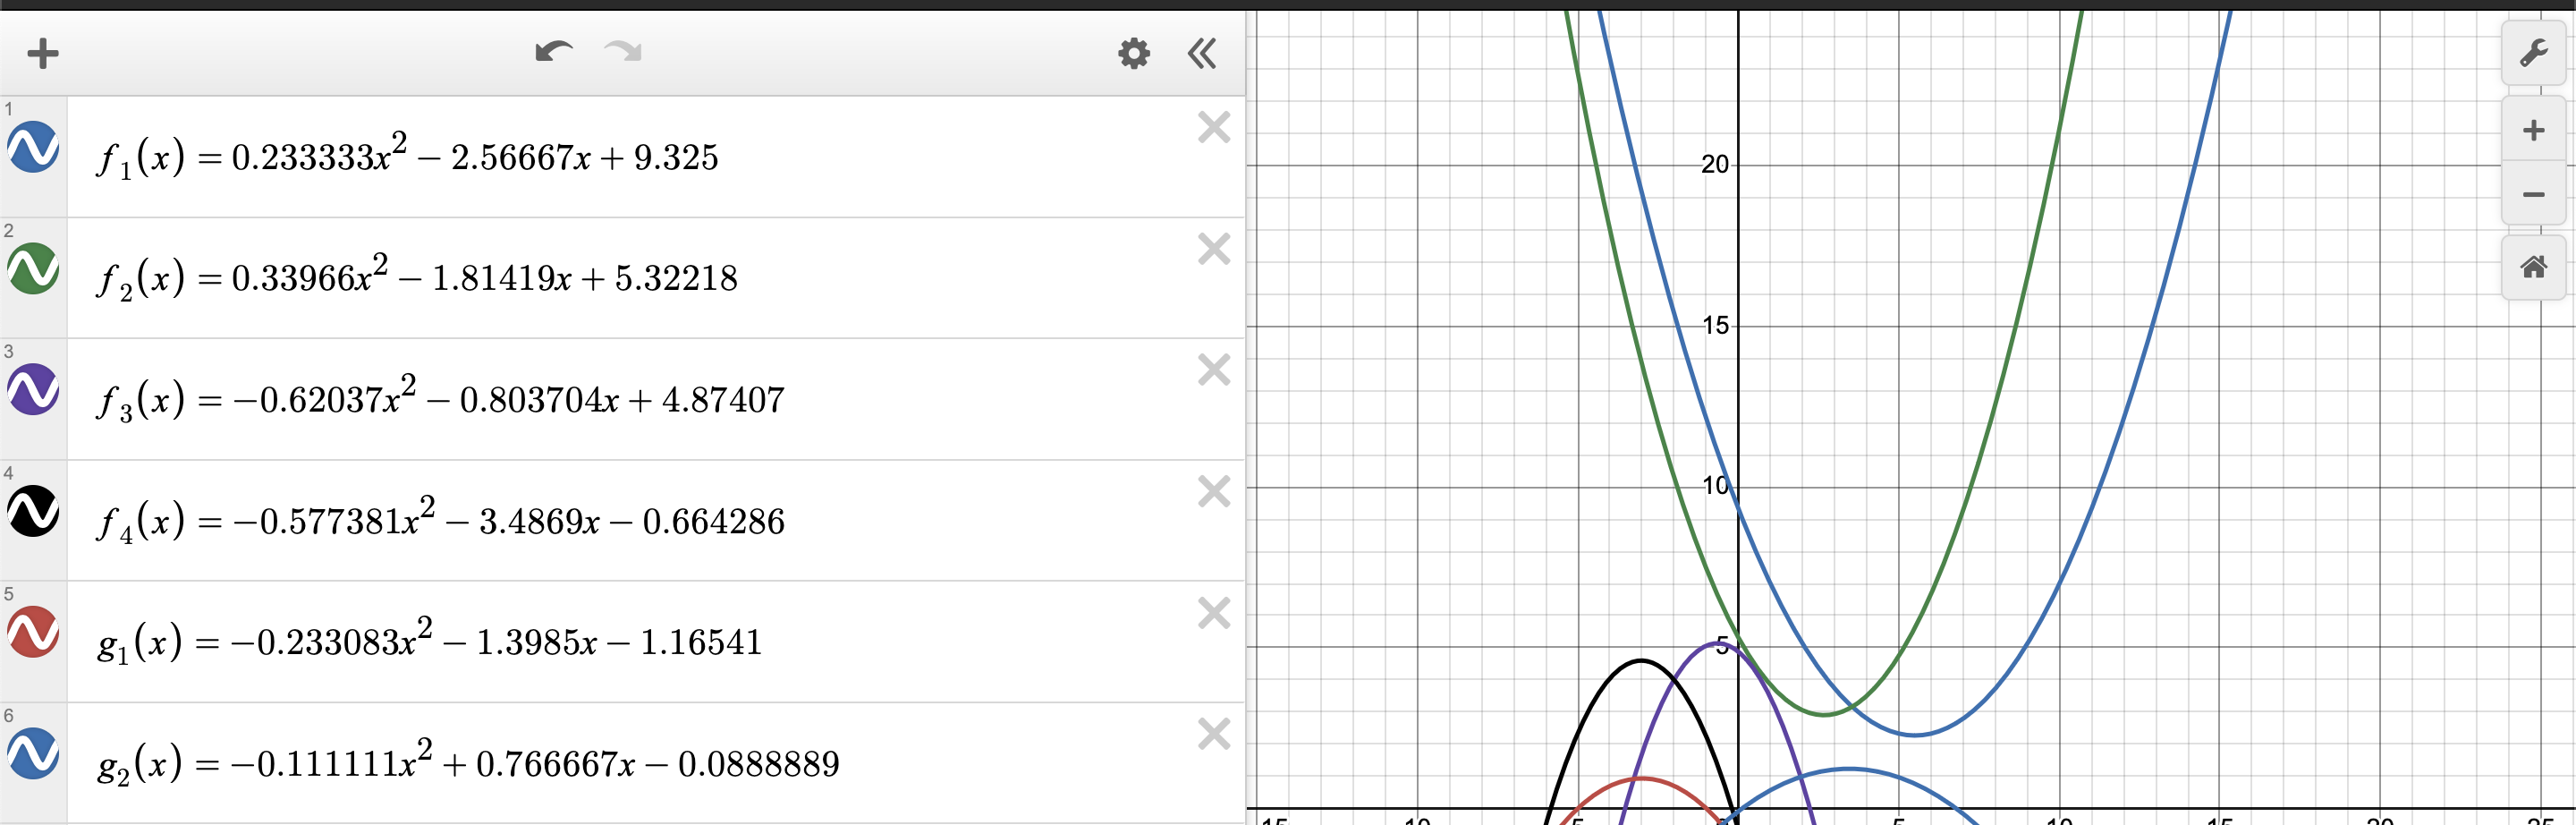
\includegraphics[width=1\linewidth]{media/ia-check-2.png}
\end{figure}
\begin{figure}[H]
    \centering
    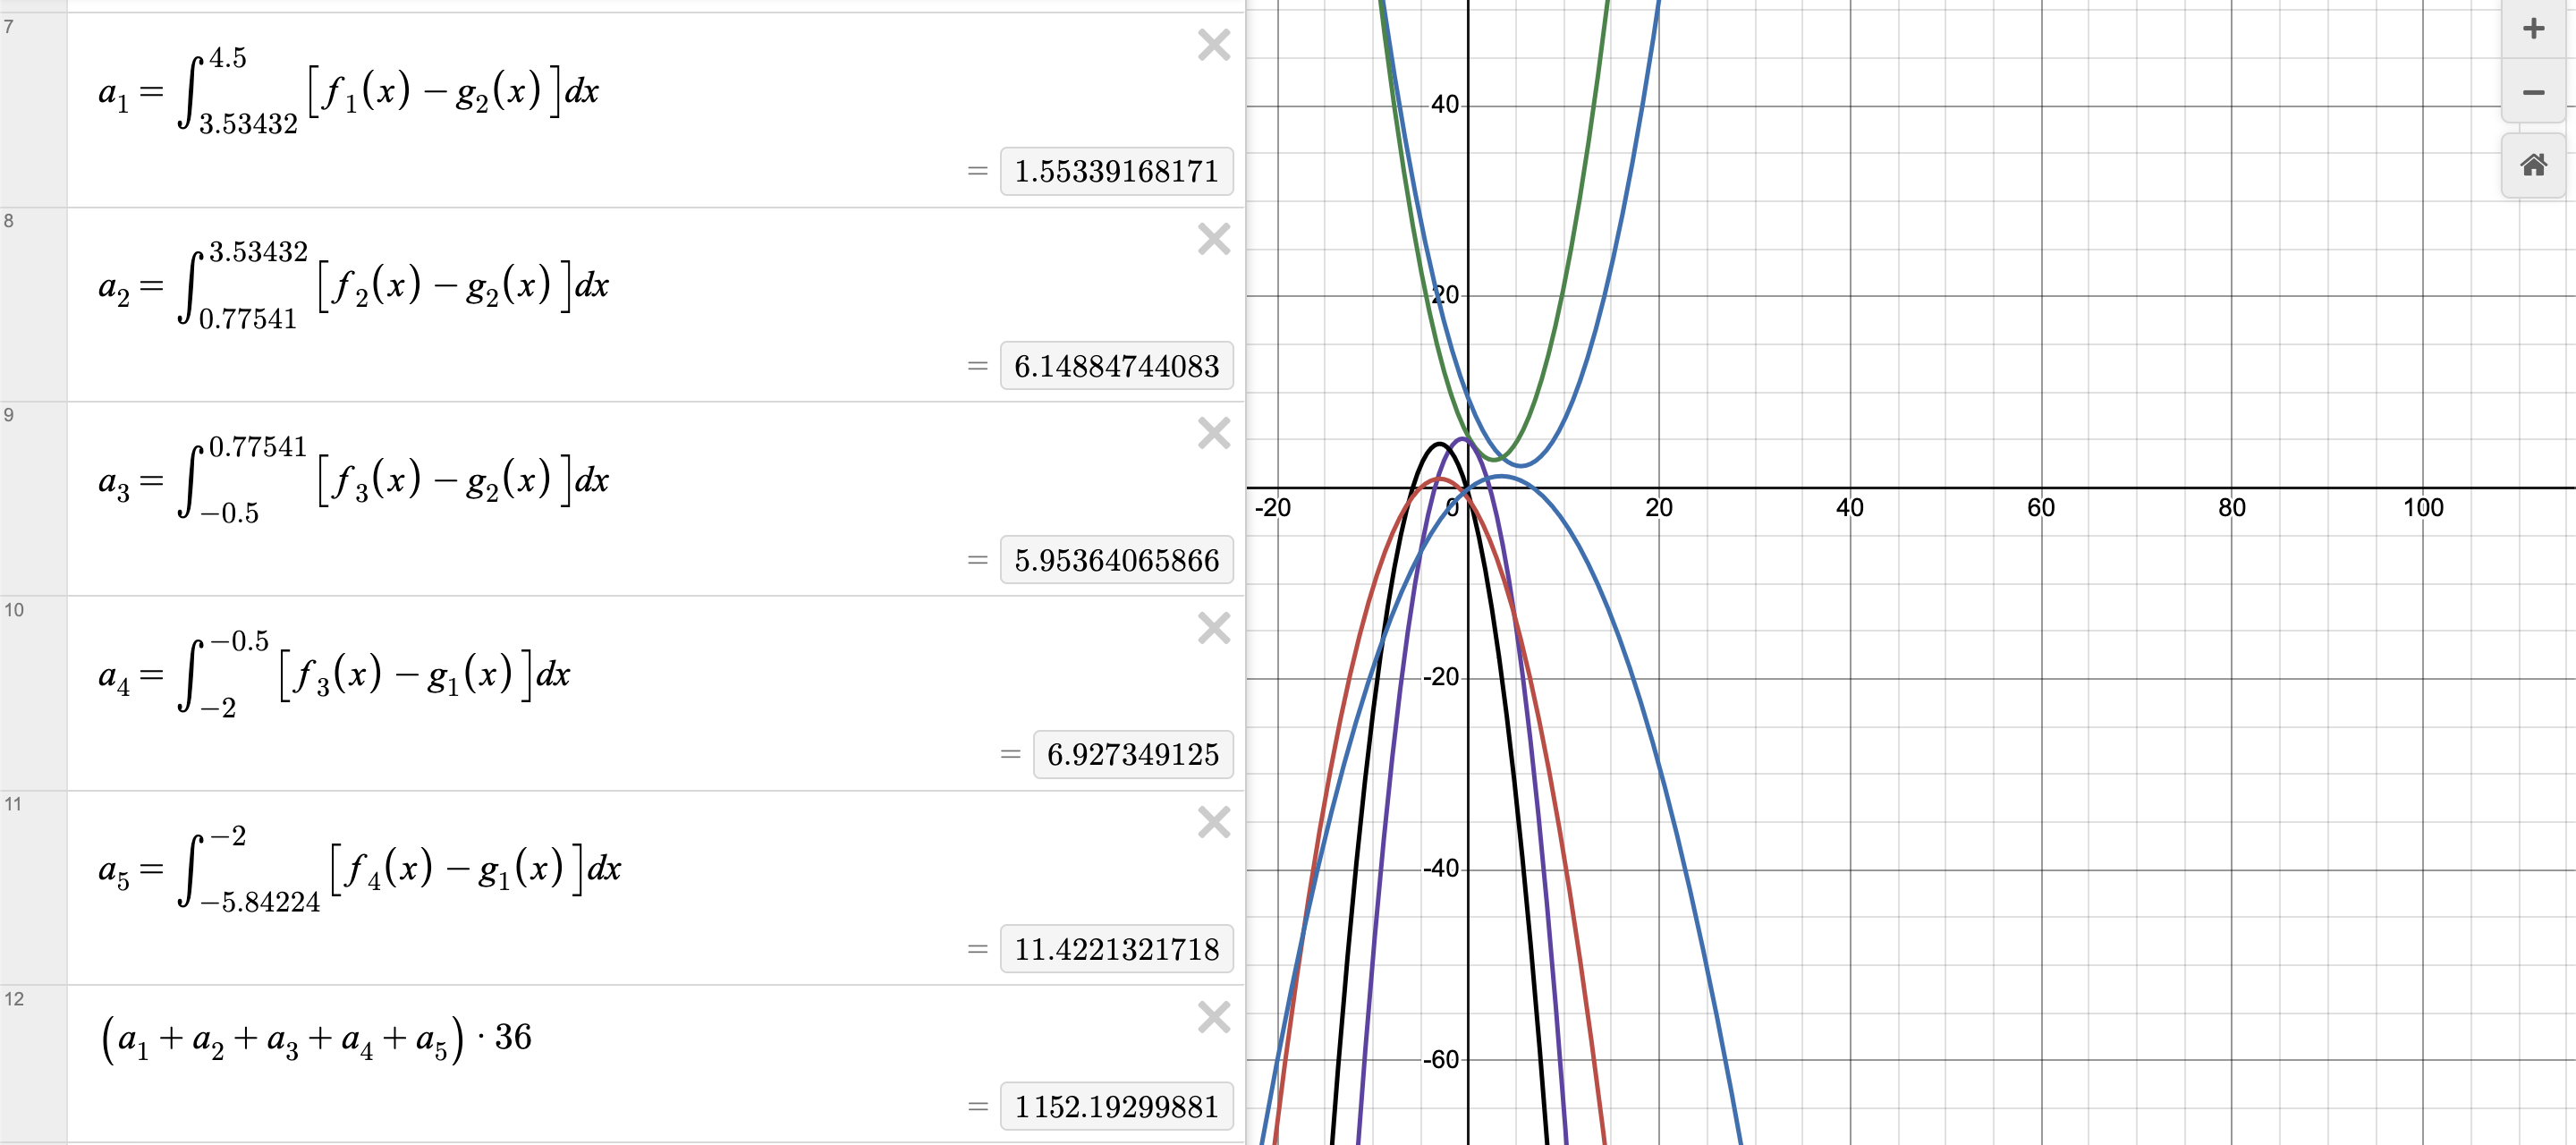
\includegraphics[width=1\linewidth]{media/ia-check-1.png}
\end{figure}

\newpage
\RaggedRight
\printbibliography
\bgroup
\singlespacing
\begin{flushright}
\footnotesize
\vspace{-8pt}
\textbf{2608 words}
\end{flushright}
\egroup
%TC:endignore
\end{document}
